%==============================================================================
%  Convolutional Neural Networks for Earth Observation
%  A Student Reference Textbook
%==============================================================================
\documentclass[11pt,openany]{book}

\usepackage[a4paper,margin=2.4cm,headheight=14pt]{geometry}
\usepackage[T1]{fontenc}
\usepackage{lmodern}
\usepackage{microtype}
\usepackage{amsmath,amssymb,amsthm}
\usepackage{mathtools}
\usepackage{graphicx}
\usepackage{xcolor}
\usepackage{booktabs}
\usepackage{tabularx}
\usepackage{array}
\usepackage{caption}
\usepackage{subcaption}
\usepackage{enumitem}
\usepackage{tikz}
\usetikzlibrary{positioning,arrows.meta,calc,fit,backgrounds,shapes.geometric}
\usepackage[most]{tcolorbox}
\usepackage{listings}
\usepackage{seqsplit}
\usepackage{fancyhdr}
\usepackage{titlesec}
\usepackage[hidelinks,colorlinks=true,linkcolor=eoblue,citecolor=eogreen,urlcolor=eoblue]{hyperref}

%------------------------------------------------------------------ colours
\definecolor{eoblue}{HTML}{1E56C8}
\definecolor{eogreen}{HTML}{1A7A1A}
\definecolor{eoearth}{HTML}{A0754A}
\definecolor{eored}{HTML}{E30B0B}
\definecolor{eodark}{HTML}{1F2A44}
\definecolor{codebg}{HTML}{F5F6F8}
\definecolor{codekw}{HTML}{0B5394}
\definecolor{codestr}{HTML}{1A7A1A}
\definecolor{codecom}{HTML}{7A7A7A}
\definecolor{lightgray}{HTML}{ECEFF3}

%------------------------------------------------------------------ headers
\pagestyle{fancy}
\fancyhf{}
\renewcommand{\headrulewidth}{0.4pt}
\fancyhead[LE]{\small\nouppercase{\leftmark}}
\fancyhead[RO]{\small\nouppercase{\rightmark}}
\fancyfoot[C]{\thepage}
\fancypagestyle{plain}{\fancyhf{}\fancyfoot[C]{\thepage}\renewcommand{\headrulewidth}{0pt}}

%------------------------------------------------------------------ chapter title format
\titleformat{\chapter}[display]
  {\normalfont\huge\bfseries\color{eodark}}
  {\filright\Large\color{eoblue}Chapter \thechapter}{0.6ex}{\Huge\raggedright}
\titlespacing*{\chapter}{0pt}{10pt}{24pt}

%------------------------------------------------------------------ code listing style
\lstdefinestyle{py}{
  language=Python,
  backgroundcolor=\color{codebg},
  basicstyle=\ttfamily\small,
  keywordstyle=\color{codekw}\bfseries,
  stringstyle=\color{codestr},
  commentstyle=\color{codecom}\itshape,
  numberstyle=\tiny\color{codecom},
  numbers=left,
  numbersep=8pt,
  frame=single,
  rulecolor=\color{lightgray},
  framesep=6pt,
  breaklines=true,
  showstringspaces=false,
  columns=fullflexible,
  keepspaces=true,
  literate={\ }{{\ }}1,
  morekeywords={self,nn,torch,np,F,with,as,assert}
}
\lstset{style=py}

%------------------------------------------------------------------ boxes
\newtcolorbox{objbox}{colback=eoblue!5,colframe=eoblue!70,boxrule=0.7pt,
  arc=2pt,left=8pt,right=8pt,top=6pt,bottom=6pt,
  title=\textbf{Learning Objectives},fonttitle=\color{white},
  coltitle=white,colbacktitle=eoblue!80}

\newtcolorbox{keybox}{colback=eogreen!6,colframe=eogreen!60,boxrule=0.7pt,
  arc=2pt,left=8pt,right=8pt,top=6pt,bottom=6pt,
  title=\textbf{Key Concepts},coltitle=white,colbacktitle=eogreen!70}

\newtcolorbox{practbox}{colback=eoearth!8,colframe=eoearth!70,boxrule=0.7pt,
  arc=2pt,left=8pt,right=8pt,top=6pt,bottom=6pt,
  title=\textbf{Practical Session},coltitle=white,colbacktitle=eoearth!80}

\newtcolorbox{exbox}{colback=gray!5,colframe=gray!55,boxrule=0.7pt,
  arc=2pt,left=8pt,right=8pt,top=6pt,bottom=6pt,
  title=\textbf{Exercises \& Mini-Project},coltitle=white,colbacktitle=gray!60}

\newtcolorbox{notebox}[1][Note]{colback=eored!4,colframe=eored!55,boxrule=0.6pt,
  arc=2pt,left=8pt,right=8pt,top=5pt,bottom=5pt,
  title=\textbf{#1},coltitle=white,colbacktitle=eored!65}

% chapter metadata strip
\newcommand{\chapmeta}[3]{%
  \begin{center}\small
  \fcolorbox{lightgray}{lightgray}{\parbox{0.98\linewidth}{\centering
  \textbf{Difficulty:} #1 \quad$\bullet$\quad \textbf{Duration:} #2 \quad$\bullet$\quad \textbf{Datasets:} #3}}
  \end{center}\vspace{4pt}}

\newcommand{\R}{\mathbb{R}}
\newcommand{\E}{\mathbb{E}}

% breakable monospace path macro for long file paths (body text only)
\newcommand{\nbpath}[1]{\texttt{\seqsplit{#1}}}
% wide diagrams scaled to fit the text width
\newcommand{\fitwidth}[1]{\resizebox{\linewidth}{!}{#1}}

\theoremstyle{definition}
\newtheorem{example}{Example}[chapter]

%==============================================================================
\begin{document}
\frontmatter

%------------------------------------------------------------------ title page
\begin{titlepage}
\centering
\vspace*{1.5cm}
{\color{eoblue}\rule{\linewidth}{1.5pt}}\\[6pt]
{\Huge\bfseries\color{eodark} Convolutional Neural Networks\\[4pt] for Earth Observation}\\[10pt]
{\Large A Student Reference Textbook}\\[6pt]
{\large\itshape From CNN fundamentals to full geospatial deep-learning pipelines}\\[4pt]
{\color{eoblue}\rule{\linewidth}{1.5pt}}\\[1.4cm]

\begin{tikzpicture}
  \def\n{7}
  \foreach \i/\c in {0/eoblue,1/eogreen,2/eoearth,3/eored,4/eodark,5/eoblue,6/eogreen}{
    \fill[\c!70] (\i*0.9,0) rectangle ++(0.8,0.8);
  }
  \node[white,font=\small\bfseries] at (3.15,0.4) {SENTINEL-2};
\end{tikzpicture}\\[1.4cm]

{\large Backbone project:\\[2pt]\textbf{Sentinel-2 Multiclass Land-Cover Segmentation}}\\[1.2cm]

{\large A production-grade course for advanced Python programmers\\ entering computer vision and remote sensing}\\[2cm]

{\large Companion to the 12-chapter notebook series and the \texttt{eo\_cnn} reference package}\\[0.6cm]
{\small Edition 1.0 \quad$\cdot$\quad MIT License (materials)}
\vfill
\end{titlepage}

\tableofcontents

%------------------------------------------------------------------ preface
\chapter*{Preface}
\addcontentsline{toc}{chapter}{Preface}
\markboth{Preface}{Preface}

This book is the written reference for the course \emph{Convolutional Neural
Networks for Earth Observation}. It is designed for a reader who is already an
experienced software engineer and who has trained neural networks before, but
who has only seen convolutional networks in theory and has little exposure to
satellite imagery. The goal is not to be an encyclopedia of deep learning;
it is to take you, chapter by chapter, from the convolution operation to a
deployable system that turns a raw Sentinel-2 scene into a georeferenced
land-cover map.

\paragraph{Why a single backbone project.}
Many courses teach CNNs through a scatter of unrelated toy datasets. This one
is deliberately built around \emph{one} cohesive arc: land-cover mapping. We
begin with patch classification on EuroSAT, where the machinery is simplest,
then graduate to dense pixel-level prediction (semantic segmentation) on
LoveDA and synthetic Sentinel-2 scenes, and finally assemble a complete
inference pipeline. Every concept introduced for classification --- the
encoder, the loss, transfer learning, augmentation --- is reused and extended
for segmentation. The continuity is the pedagogy.

\paragraph{How to read this book.}
Each chapter opens with explicit learning objectives, a difficulty/duration
strip, and the datasets it uses. The body develops the theory with the
mathematics written out properly, and closes with a \emph{Practical Session}
box that mirrors the corresponding Jupyter notebook, followed by exercises and
a mini-project. The mathematics is meant to be read with a pencil; the
practical boxes are meant to be read with a keyboard. You will get the most
out of the book by running the matching notebook (\texttt{notebooks/chapter\_NN\_*})
immediately after each chapter.

\paragraph{Notation.}
Tensors are written as multidimensional arrays with shape conventions in the
PyTorch order $(N, C, H, W)$ --- batch, channels, height, width. Scalars are
lower-case italic ($x$), vectors bold lower-case ($\mathbf{x}$), matrices and
tensors upper-case ($K$, $I$). A convolution layer is denoted $*$ even though,
as we will see in Chapter~2, frameworks implement cross-correlation. Spectral
bands are referenced by their Sentinel-2 names (B02, B03, $\dots$, B12).

\paragraph{Software.}
All code targets Python~3.12 with PyTorch~$\geq$~2.2, \texttt{torchgeo},
\texttt{rasterio}, \nbpath{segmentation-models-pytorch}, and
\texttt{albumentations}. Every notebook runs on Google Colab's free T4 GPU and
falls back to CPU through a \texttt{FAST\_MODE} flag. Appendix~A gives the full
environment setup; Appendix~B lists papers, tools and datasets.

\vspace{1em}
\noindent\emph{A note on figures.} Several figures in this book are generated
programmatically (script \nbpath{docs/textbook/make\_figures.py}) from the same
NumPy/Matplotlib stack used in the practicals, so you can reproduce and modify
them yourself.

%------------------------------------------------------------------ introduction
\chapter*{Introduction: Choosing the Backbone Project}
\addcontentsline{toc}{chapter}{Introduction: Choosing the Backbone Project}
\markboth{Introduction}{Introduction}

Before the first line of code, a curriculum designer must answer one question:
\emph{which problem should the whole course be built around?} The choice
determines which CNN concepts can be taught organically and which must be
bolted on artificially. Three candidate Earth-Observation (EO) projects were
evaluated.

\section*{The three candidates}

\paragraph{Project 1 --- EuroSAT land-use classification.}
Classify $64\times64$ Sentinel-2 patches into one of ten land-use classes.
The dataset (27{,}000 patches, RGB or 13-band, $\sim$90\,MB) downloads in one
\texttt{torchgeo} call. It is the ``MNIST of EO'': clean, balanced, and fast
on CPU. It is \emph{ideal} for teaching the classification machinery ---
softmax, cross-entropy, accuracy, training loops --- but it teaches no spatial
prediction, no geospatial context, and no encoder--decoder design. Difficulty:
beginner.

\paragraph{Project 2 --- SpaceNet building-footprint extraction.}
Binary segmentation of buildings from 30\,cm very-high-resolution imagery with
polygon labels. Strongly motivating and visually satisfying, but the dataset is
$\sim$24\,GB, requires AWS tooling, uses proprietary Maxar imagery, and demands
heavy polygon-to-raster preprocessing before any training. The binary task also
limits architectural variety. Difficulty: intermediate to advanced; poor
classroom accessibility.

\paragraph{Project 3 --- Sentinel-2 multiclass land-cover segmentation.}
Assign every pixel a land-cover class (urban, agriculture, forest, grassland,
water, bare soil, $\dots$) from multispectral 10\,m imagery, using LoveDA
(auto-downloaded via \texttt{torchgeo}, $\sim$3\,GB) and synthetic/real
Sentinel-2 scenes. It exercises the \emph{entire} CNN curriculum --- spatial
convolution, pooling, skip connections, transfer learning, augmentation,
dense-prediction losses and metrics --- and all EO-specific skills: multi-band
loading, spectral indices, normalization, tiling, sliding-window inference, and
GeoTIFF export. Difficulty: intermediate to advanced, with a beginner on-ramp
through EuroSAT.

\section*{Comparative evaluation}

\begin{center}\small
\renewcommand{\arraystretch}{1.25}
\begin{tabularx}{\linewidth}{@{}lXXX@{}}
\toprule
\textbf{Criterion} & \textbf{EuroSAT} & \textbf{SpaceNet} & \textbf{S2 land cover}\\
\midrule
Task type & Classification & Binary segmentation & \textbf{Multiclass seg.}\\
Educational breadth & Narrow & Medium & \textbf{Wide}\\
Dataset access & Excellent (90\,MB) & Poor (24\,GB, AWS) & \textbf{Excellent (3\,GB)}\\
Annotation quality & Excellent & Variable & Good (expert)\\
Compute needs & Very low & High & Medium (GPU)\\
Geospatial preproc. & None & Medium & \textbf{Full}\\
Visual output & Low & Medium & \textbf{High}\\
Transfer-learning demo & Good & Good & \textbf{Excellent}\\
Augmentation relevance & Low & Medium & \textbf{High}\\
Industry relevance & Medium & High & \textbf{Highest}\\
Beginner friendliness & \textbf{Excellent} & Poor & Good\\
Full pipeline & No & Partial & \textbf{Yes}\\
Architecture diversity & Low & Medium & \textbf{High}\\
Multi-band / indices & MS variant & No & \textbf{Yes}\\
\midrule
\textbf{Overall (1--10)} & 7 & 6 & \textbf{9}\\
\bottomrule
\end{tabularx}
\end{center}

\section*{Decision}

The backbone of this course is \textbf{Sentinel-2 multiclass land-cover
segmentation}. It is the only candidate that sustains a coherent twelve-chapter
arc without an awkward pivot: EuroSAT classification provides the beginner
on-ramp (Chapters 5--8), the same encoder is reused inside a U-Net for
segmentation (Chapters 9--10), and the course culminates in full-scene
inference and a GeoTIFF map (Chapters 11--12 and the capstone). It mirrors real
production systems --- ESA WorldCover, Google Dynamic World, Planet NICFI ---
so the skills transfer directly to industry. SpaceNet's data friction and
EuroSAT's pedagogical ceiling rule them out as \emph{sole} backbones, though
EuroSAT serves perfectly as the introductory vehicle inside this larger arc.

\begin{center}
\begin{tikzpicture}[font=\small,node distance=6mm]
  \tikzstyle{b}=[draw,rounded corners,minimum height=9mm,minimum width=30mm,align=center,fill=eoblue!8]
  \node[b] (a) {EuroSAT\\classification\\\scriptsize(Ch.\,5--8)};
  \node[b,right=14mm of a,fill=eogreen!10] (c) {U-Net binary/\\multiclass seg.\\\scriptsize(Ch.\,9--10)};
  \node[b,right=14mm of c,fill=eoearth!12] (d) {Full-scene\\GeoTIFF pipeline\\\scriptsize(Ch.\,11--12, cap.)};
  \draw[-{Latex},thick] (a)--(c);
  \draw[-{Latex},thick] (c)--(d);
\end{tikzpicture}
\end{center}

\noindent The shared encoder is the thread: only the decoder head changes as we
move from classification to dense prediction.

\mainmatter

\part{Foundations: From Pixels to Convolutions}
\chapter{Introduction: Earth Observation and Deep Learning}
\label{ch:intro}

\chapmeta{Beginner}{$\sim$4\,h (2\,h theory + 2\,h practical)}{EuroSAT RGB (torchgeo, $\sim$90\,MB)}

\begin{objbox}
\begin{itemize}[leftmargin=1.2em,nosep]
  \item Understand what satellite imagery is and why it matters for AI.
  \item Load and visualise multi-band GeoTIFF files with \texttt{rasterio}.
  \item Understand spectral bands, spatial resolution, and coordinate reference systems (CRS).
  \item Explore the structure of the EuroSAT benchmark dataset.
  \item Build intuition for why CNNs --- not per-pixel classifiers --- extract land-use information.
\end{itemize}
\end{objbox}

\section{What is Earth Observation?}

Earth Observation (EO) is the systematic collection of information about the
Earth's physical, chemical and biological systems using remote sensors, chiefly
satellites. Unlike a consumer camera, an EO sensor does not produce a
``photograph''; it measures the intensity of electromagnetic radiation
reflected or emitted by the surface within a set of narrow wavelength intervals
called \emph{spectral bands}. Each band is itself a grey-scale image, so a
single acquisition is a stack of co-registered images --- a tensor of shape
$(C, H, W)$ where $C$ is the number of bands. This structural identity with the
input a CNN expects is the reason deep learning transferred so naturally to
remote sensing.

Four properties characterise any EO sensor and constrain the models we build on
top of it:
\begin{description}[leftmargin=1.6em,style=nextline]
  \item[Spatial resolution] the ground area covered by one pixel (the
  ground-sampling distance, GSD). Sentinel-2 is 10--60\,m; WorldView-3 reaches
  0.3\,m.
  \item[Spectral resolution] the number and width of the bands. More bands
  reveal more about surface chemistry (e.g.\ chlorophyll, moisture).
  \item[Temporal resolution] the revisit period. Sentinel-2 revisits every
  $\sim$5 days, enabling change-detection and time-series tasks.
  \item[Radiometric resolution] the bit depth of the measurement (Sentinel-2
  stores 12-bit reflectance scaled to integers).
\end{description}

\begin{center}\small
\renewcommand{\arraystretch}{1.15}
\begin{tabular}{@{}lllll@{}}
\toprule
Satellite & Operator & Resolution & Revisit & Bands\\
\midrule
Sentinel-2 & ESA & 10--60\,m & 5\,days & 13\\
Landsat 8/9 & USGS/NASA & 30\,m & 16\,days & 11\\
WorldView-3 & Maxar & 0.3\,m & 1\,day & 29\\
Planet NICFI & Planet & 4.77\,m & daily & 4\\
\bottomrule
\end{tabular}
\end{center}

Resolution drives architecture. At 10\,m/px a single Sentinel-2 pixel covers a
tennis court, so individual buildings are sub-pixel; at 0.3\,m/px cars and tree
crowns are resolved. The size of the objects you care about, measured in
pixels, must fit inside the network's receptive field (Chapter~\ref{ch:conv}).

\section{Spectral bands: what satellites measure}

The single most important EO concept for a newcomer is that \emph{each band is
an image}, and different materials have characteristic \emph{spectral
signatures} --- reflectance as a function of wavelength. Figure~\ref{fig:spec}
shows idealised signatures for four land-cover types across the Sentinel-2
bands.

\begin{figure}[h]
\centering
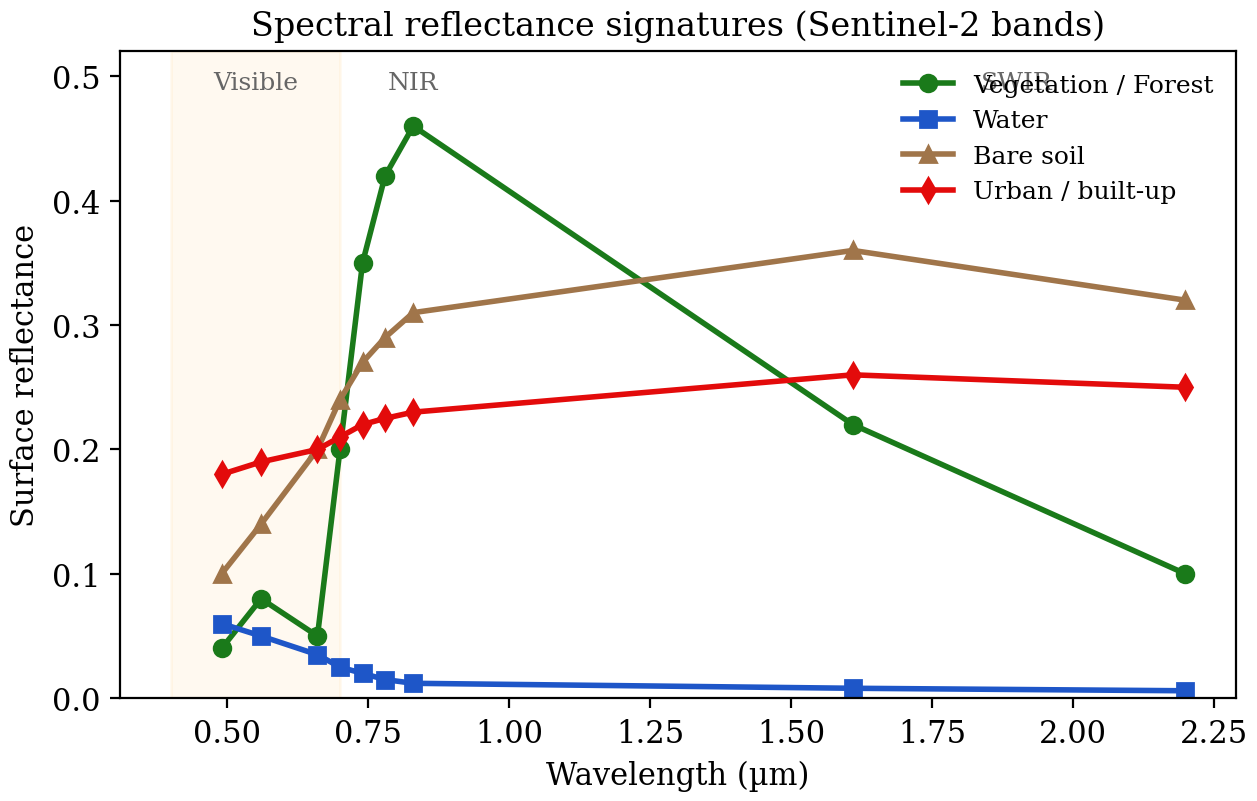
\includegraphics[width=0.82\linewidth]{figures/spectral_signatures.png}
\caption{Spectral reflectance signatures. Healthy vegetation reflects strongly
in the near-infrared (NIR, B08) and absorbs in the red (B04); water absorbs
almost everything beyond the visible; soil rises gently toward the SWIR. These
contrasts are exactly what spectral indices and CNNs exploit.}
\label{fig:spec}
\end{figure}

The vegetation ``red edge'' --- the steep rise between B04 (red) and B08 (NIR)
--- underlies the most famous remote-sensing index, the Normalised Difference
Vegetation Index:
\begin{equation}
\mathrm{NDVI} = \frac{\rho_\mathrm{NIR}-\rho_\mathrm{Red}}{\rho_\mathrm{NIR}+\rho_\mathrm{Red}}
= \frac{\mathrm{B08}-\mathrm{B04}}{\mathrm{B08}+\mathrm{B04}} \in [-1,1].
\label{eq:ndvi}
\end{equation}
Dense vegetation gives $\mathrm{NDVI}\gtrsim 0.6$; water gives negative values.
We will compute indices like this in Chapter~\ref{ch:preproc} and feed them as
extra channels to networks.

\begin{notebox}[Common pitfall]
Reflectance values are not 8-bit ``pixels''. Sentinel-2 Level-2A products store
bottom-of-atmosphere reflectance as integers (e.g.\ $0$--$10000$). Forgetting to
scale and normalise these before feeding a network is the single most frequent
beginner error (Chapter~\ref{ch:preproc}).
\end{notebox}

\section{Raster and vector data}

GIS data comes in two forms. \emph{Raster} data is a grid of pixels with a
geotransform mapping pixel $(row,col)$ to a world coordinate, plus a CRS
(coordinate reference system, e.g.\ EPSG:32633 for UTM zone 33N). Satellite
imagery and our prediction maps are rasters, read and written with
\texttt{rasterio}. \emph{Vector} data is geometry --- points, lines, polygons
--- stored in shapefiles or GeoJSON and manipulated with \texttt{geopandas};
building footprints and OpenStreetMap labels are vectors. Training a
segmentation model usually means \emph{rasterising} vector labels onto the same
grid as the imagery.

\section{The EuroSAT dataset}

EuroSAT (Helber et al., 2019) is the benchmark we use to learn the
classification machinery. It contains 27{,}000 Sentinel-2 patches of
$64\times64$ pixels, each labelled with one of ten land-use classes:
\textsf{AnnualCrop, Forest, HerbaceousVegetation, Highway, Industrial,
Pasture, PermanentCrop, Residential, River, SeaLake}. Two variants exist: RGB
(3 bands) and multispectral (13 bands). It is clean, balanced
($\sim$2000--3000 samples/class) and downloads in one line via
\texttt{torchgeo}, which makes it perfect for fast iteration --- but note that a
patch-level label teaches \emph{classification only}; it cannot teach the
spatial prediction we build toward later.

\section{Why CNNs, not per-pixel classifiers?}

Classical remote sensing classified each pixel independently from its spectral
vector using SVMs or random forests. This ignores \emph{spatial context}.
Consider the visual texture of land cover: forests have a rough, self-similar
canopy; urban areas show grid-like street patterns and high local heterogeneity;
water is smooth and homogeneous; agriculture shows regular field boundaries and
row striping. None of these are visible to a per-pixel method, because they live
in the \emph{neighbourhood} of a pixel, not in the pixel itself. A convolutional
network learns spatial filters that respond to exactly such patterns, and
stacks them into a hierarchy --- the subject of the next three chapters.

\begin{keybox}
\begin{itemize}[leftmargin=1.2em,nosep]
  \item Each spectral band is an image; an acquisition is a $(C,H,W)$ tensor.
  \item Spectral signatures distinguish materials; indices such as NDVI
  (Eq.~\ref{eq:ndvi}) summarise them.
  \item Reflectance must be scaled and normalised before training.
  \item Raster (pixels + CRS) vs vector (geometry); labels are often rasterised.
  \item CNNs learn \emph{spatial} patterns that per-pixel classifiers miss.
\end{itemize}
\end{keybox}

\begin{practbox}
Notebook: \nbpath{notebooks/chapter\_01\_intro\_eo\_dl/01\_practical\_eo\_data\_exploration.ipynb}.
\begin{enumerate}[leftmargin=1.4em,nosep]
  \item Run the Colab/environment setup cell; confirm \texttt{DEVICE} and
  \texttt{FAST\_MODE} are detected.
  \item Download EuroSAT RGB via \texttt{torchgeo} and visualise one sample per
  class in a $2\times5$ grid.
  \item Inspect the class distribution as a bar chart; confirm the dataset is
  near-balanced.
  \item Read a multi-band GeoTIFF with \texttt{rasterio}; print its shape, dtype,
  CRS and geotransform; render a true-colour composite from B04/B03/B02.
  \item Compute and display NDVI for a vegetated and a water sample.
\end{enumerate}
A representative skeleton for reading a scene and computing an index:
\begin{lstlisting}
import rasterio, numpy as np
with rasterio.open(path) as src:
    img = src.read().astype("float32")   # (C, H, W)
    print(img.shape, src.crs, src.transform)
red, nir = img[3], img[7]                  # B04, B08 (0-indexed)
ndvi = (nir - red) / (nir + red + 1e-6)
\end{lstlisting}
\end{practbox}

\begin{exbox}
\textbf{1.1 Channel statistics.} Over the EuroSAT test split, compute the per-channel
mean and standard deviation. Tabulate them --- these become your normalization
constants in Chapter~\ref{ch:classif}.\\[2pt]
\textbf{1.2 Spectral profiles.} For five random samples from each class, plot the
mean reflectance vs band number. Verify water has near-zero NIR/SWIR and forest
has high NIR.\\[2pt]
\textbf{1.3 NDVI thresholding.} Using EuroSAT-MS, compute NDVI for three
\textsf{Forest} and three \textsf{SeaLake} samples; find a threshold separating
them.\\[2pt]
\textbf{Mini-project.} Write \texttt{describe\_sample(idx)} that prints the class
name, RGB and NIR means, and shows the RGB image beside an NDVI heatmap; run it
on five samples.
\end{exbox}

\chapter{Convolution Fundamentals}
\label{ch:conv}

\chapmeta{Beginner}{$\sim$5\,h (3\,h theory + 2\,h practical)}{EuroSAT; synthetic images}

\begin{objbox}
\begin{itemize}[leftmargin=1.2em,nosep]
  \item Define discrete 2D convolution and distinguish it from cross-correlation.
  \item Implement convolution from scratch in NumPy and reproduce \texttt{nn.Conv2d}.
  \item Derive the output-size formula for arbitrary kernel, stride and padding.
  \item Understand kernels, feature maps, weight sharing and the receptive field.
  \item Read and reason about every argument of \texttt{torch.nn.Conv2d}.
\end{itemize}
\end{objbox}

\section{The convolution operation}

A convolution slides a small array of learnable weights --- the \emph{kernel}
or \emph{filter} $K$ --- across an input image $I$ and, at each position,
computes the sum of element-wise products. The result is a \emph{feature map}.
For a single-channel input of size $H\times W$ and a kernel of size
$k\times k$, the (valid) output at position $(i,j)$ is
\begin{equation}
S[i,j] \;=\; (I * K)[i,j] \;=\; \sum_{m=0}^{k-1}\sum_{n=0}^{k-1} K[m,n]\,I[i+m,\,j+n].
\label{eq:conv}
\end{equation}
Figure~\ref{fig:conv} illustrates one such dot-product for a vertical-edge
kernel.

\begin{figure}[h]
\centering
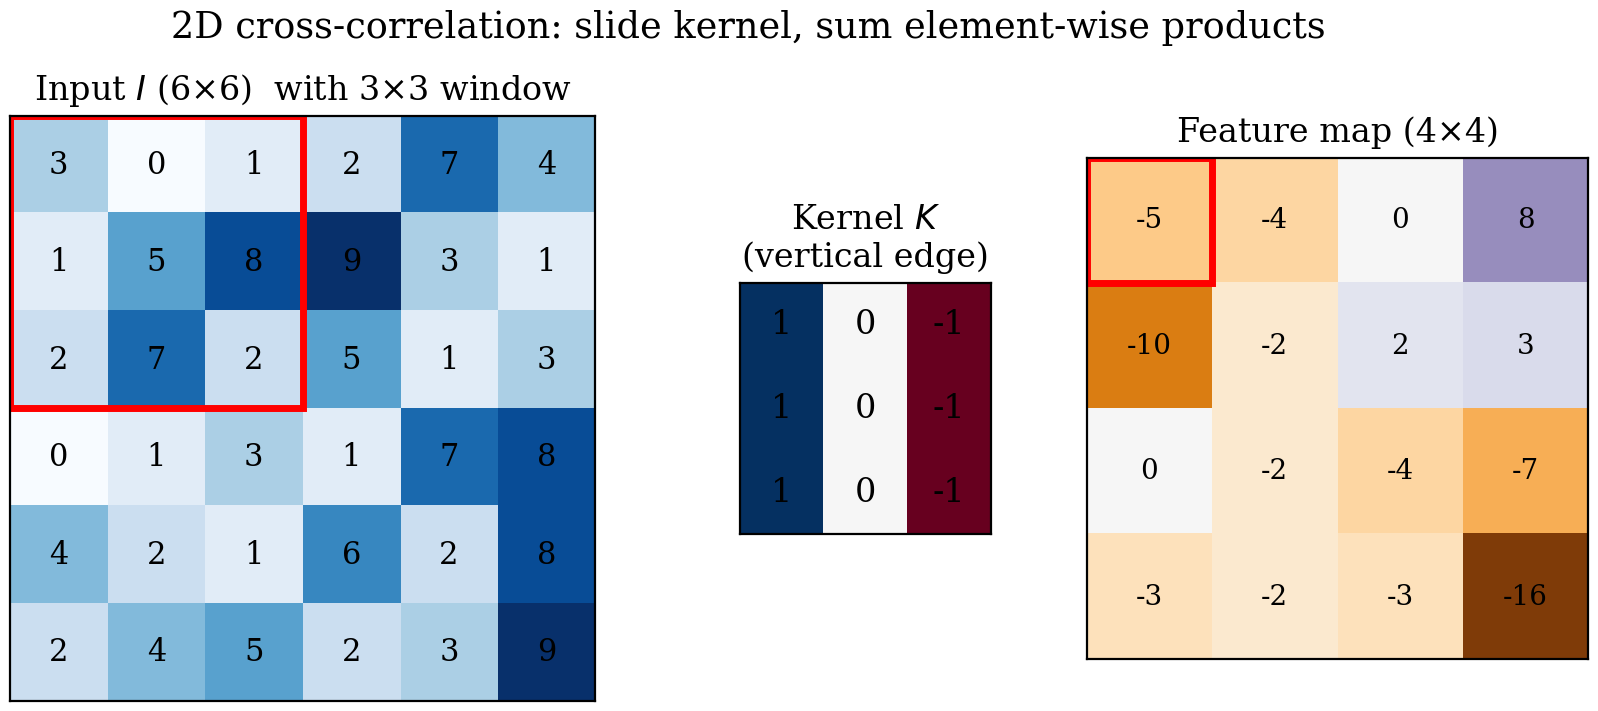
\includegraphics[width=\linewidth]{figures/convolution.png}
\caption{Discrete 2D cross-correlation. The $3\times3$ kernel (centre) is placed
at every valid position of the input (left); each placement produces one output
value (right). The same kernel is reused everywhere --- \emph{weight sharing}.}
\label{fig:conv}
\end{figure}

\paragraph{Convolution vs.\ cross-correlation.}
The mathematical convolution flips the kernel before sliding:
$(I*K)[i,j]=\sum_{m,n}K[m,n]\,I[i-m,j-n]$. Deep-learning frameworks omit the
flip and implement Eq.~\eqref{eq:conv} --- technically \emph{cross-correlation}
--- but call it ``convolution''. Because the kernel weights are learned, the
flip is irrelevant: the network simply learns the un-flipped kernel. We follow
the framework convention throughout.

\paragraph{Multi-channel convolution.}
Real inputs have $C_\mathrm{in}$ channels (3 for RGB, 13 for Sentinel-2). A
single filter then has shape $(C_\mathrm{in},k,k)$ and sums over channels; a
layer learns $C_\mathrm{out}$ such filters, producing $C_\mathrm{out}$ feature
maps:
\begin{equation}
S_o[i,j] \;=\; b_o + \sum_{c=0}^{C_\mathrm{in}-1}\sum_{m=0}^{k-1}\sum_{n=0}^{k-1}
K_o[c,m,n]\,I[c,\,i+m,\,j+n], \qquad o = 0,\dots,C_\mathrm{out}-1.
\label{eq:convmc}
\end{equation}
The weight tensor of a layer therefore has shape
$(C_\mathrm{out},C_\mathrm{in},k,k)$ and the bias has shape $(C_\mathrm{out})$.

\paragraph{Why weight sharing matters.}
A fully connected layer mapping a $64\times64\times3$ image to even $64$
hidden units needs $64\times64\times3\times64 \approx 786{,}000$ weights and is
not translation-equivariant. A convolution with $64$ filters of size
$3\times3\times3$ needs $64\times27 = 1{,}728$ weights, applies the \emph{same}
detector everywhere, and is translation-equivariant by construction. This
parameter economy and built-in spatial prior are why CNNs dominate imagery.

\section{Classic kernels: what filters detect}

Before learned filters, image processing used hand-designed kernels. They build
intuition for what a CNN's early layers discover on their own.
Figure~\ref{fig:kernels} applies several to a synthetic satellite-like scene.

\begin{figure}[h]
\centering
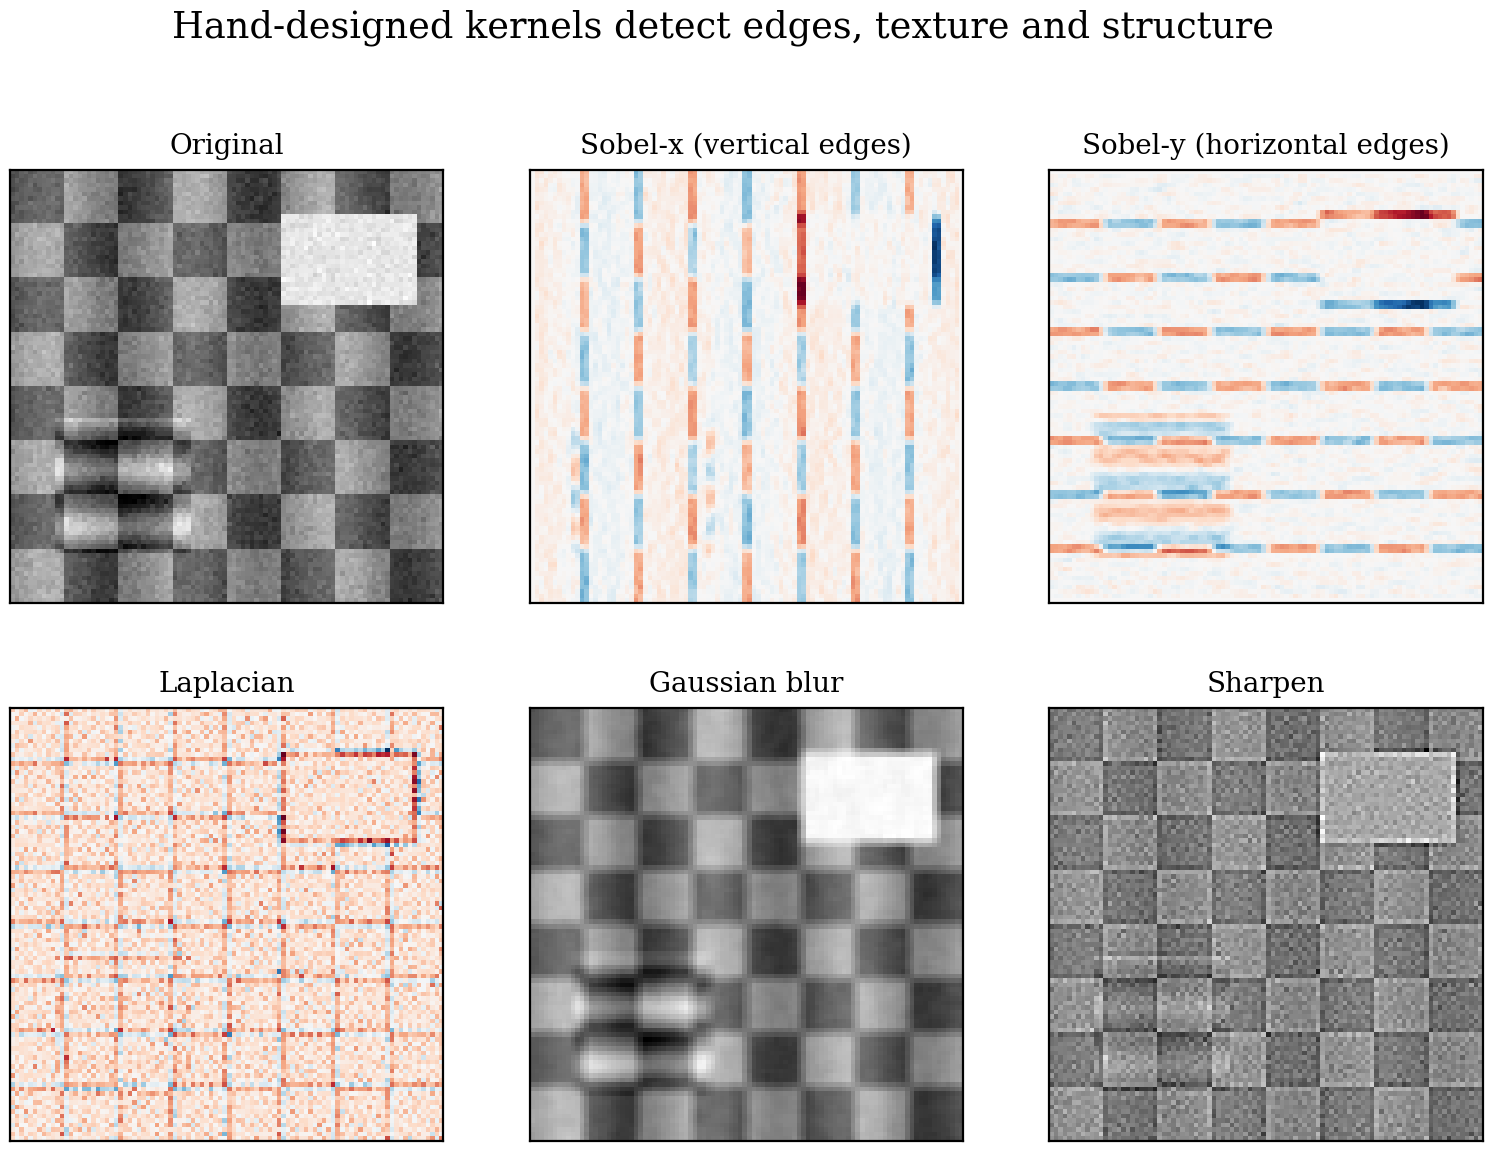
\includegraphics[width=0.95\linewidth]{figures/kernels.png}
\caption{Hand-designed kernels. Sobel filters respond to oriented edges; the
Laplacian to second-order intensity changes; Gaussian blurs; sharpening
amplifies high frequencies. Trained CNN first layers typically rediscover
edge/blob/colour-opponent filters resembling these.}
\label{fig:kernels}
\end{figure}

The horizontal Sobel kernel is
$K=\begin{psmallmatrix}1&0&-1\\2&0&-2\\1&0&-1\end{psmallmatrix}$; it
approximates $\partial I/\partial x$ and fires on vertical edges. Early CNN
layers learn Gabor-like oriented edge and colour-opponent detectors; deeper
layers combine these into textures, object parts and, eventually, semantic
concepts --- a learned hierarchy of the hand-built filters above.

\section{Padding and stride}

\paragraph{Padding.} Valid convolution shrinks the output: each spatial
dimension loses $k-1$ pixels. To keep the spatial size constant (``same''
padding) we pad the border with $p=\lfloor k/2\rfloor$ zeros on each side.

\paragraph{Stride.} The stride $s$ is the step between kernel placements. A
stride of 2 halves the output resolution, providing a learnable alternative to
pooling for downsampling.

\paragraph{Output-size formula.} For input size $n$, kernel $k$, padding $p$,
stride $s$:
\begin{equation}
n_\mathrm{out} = \left\lfloor \frac{n + 2p - k}{s} \right\rfloor + 1.
\label{eq:outsize}
\end{equation}
For $n=64$, $k=3$, $s=1$: $p=0$ gives $62$ (shrinks); $p=1$ gives $64$ (same).
With $s=2$, $k=3$, $p=1$: $n_\mathrm{out}=32$. Memorising
Eq.~\eqref{eq:outsize} prevents the most common shape-mismatch bugs.

\section{The receptive field}

The \emph{receptive field} (RF) of a unit is the region of the input image that
can influence its activation. For $N$ stacked $k\times k$ convolutions with
stride 1 and no pooling,
\begin{equation}
\mathrm{RF}_N = 1 + N\,(k-1).
\label{eq:rf}
\end{equation}
For $3\times3$ kernels: one layer sees $3$, two layers $5$, five layers $9$,
ten layers $19$. Stacking small kernels is cheaper than one large kernel for the
same RF (two $3\times3$ layers, $18$ weights/channel, match one $5\times5$,
$25$ weights) and inserts an extra non-linearity --- the design principle behind
VGG (Chapter~\ref{ch:arch}). Pooling or strided convolution multiplies the RF
growth rate (Figure~\ref{fig:rf}).

\begin{figure}[h]
\centering
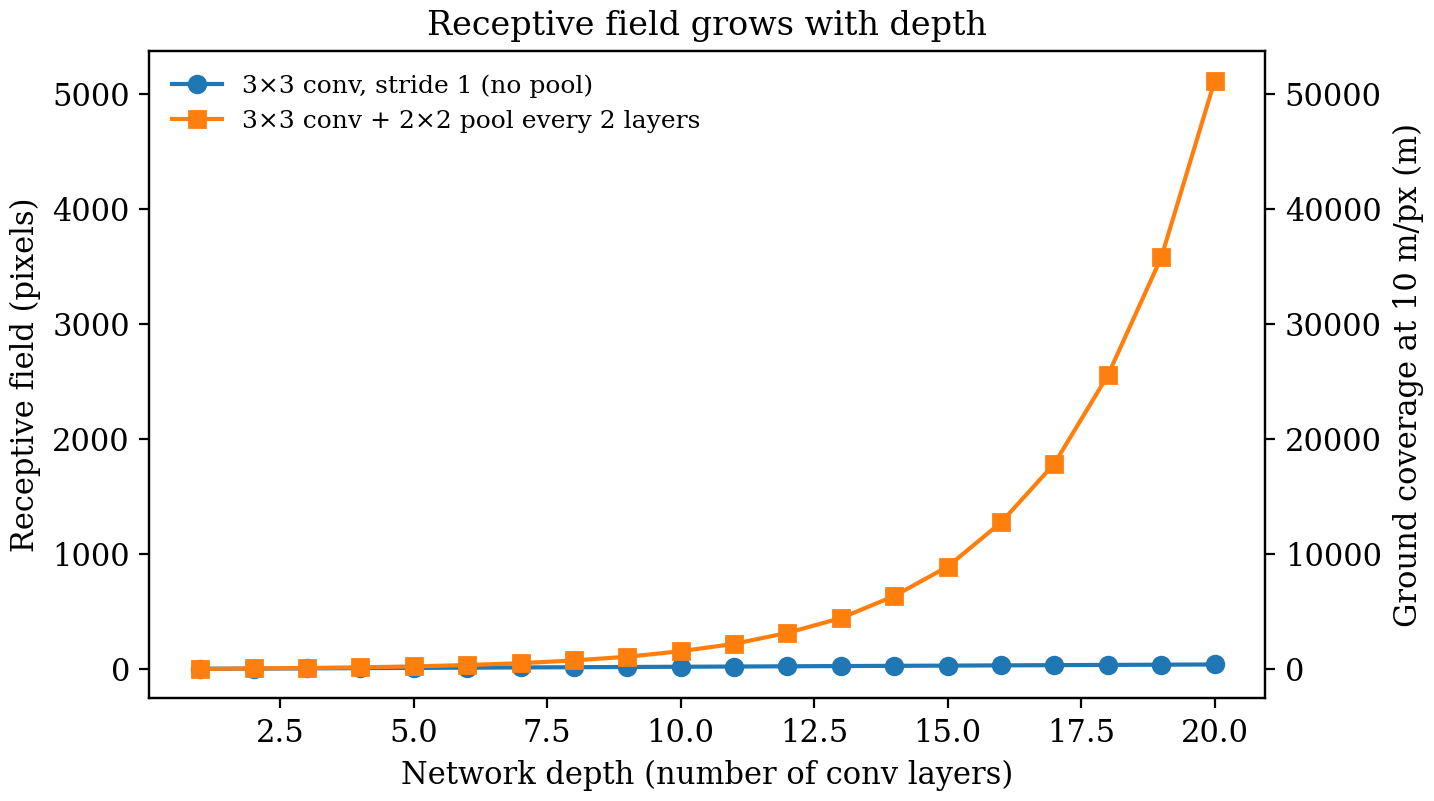
\includegraphics[width=0.72\linewidth]{figures/receptive_field.png}
\caption{Receptive field vs depth. Downsampling layers (pooling or stride~2)
make the RF grow geometrically, letting deep layers ``see'' large ground areas.
At 10\,m/px an RF of $\sim$100\,px corresponds to $\sim$1\,km --- enough to
capture field boundaries and urban blocks.}
\label{fig:rf}
\end{figure}

This is why depth lets a network detect larger objects: a unit in a deep layer
integrates information over a wide spatial extent. For EO this maps directly to
ground distance: matching the RF to the scale of your target features (a road
vs a city) is a real design decision.

\section{\texttt{nn.Conv2d} in PyTorch}

The framework layer realises Eq.~\eqref{eq:convmc}:
\begin{lstlisting}
import torch.nn as nn
conv = nn.Conv2d(in_channels=3, out_channels=32, kernel_size=3,
                 stride=1, padding=1, bias=True)
# weight shape: (out_channels, in_channels, kH, kW) = (32, 3, 3, 3)
# params: out*in*kH*kW + out = 32*3*3*3 + 32 = 896
\end{lstlisting}
Key arguments: \texttt{in\_channels} (input feature maps), \texttt{out\_channels}
(number of filters learned $=$ output maps), \texttt{kernel\_size},
\texttt{stride}, \texttt{padding}, and \texttt{bias} (set \texttt{False} when a
BatchNorm layer follows, since BN has its own shift). The parameter count of a
layer is $C_\mathrm{out}(C_\mathrm{in}\,k^2)+C_\mathrm{out}$; its cost in
multiply--accumulate operations for an $H\times W$ output is
$C_\mathrm{out}C_\mathrm{in}k^2 HW$.

\begin{keybox}
\begin{itemize}[leftmargin=1.2em,nosep]
  \item Convolution = slide kernel, sum element-wise products (Eq.~\ref{eq:conv}); frameworks skip the flip.
  \item A layer learns $C_\mathrm{out}$ filters of shape $(C_\mathrm{in},k,k)$; weight sharing gives translation equivariance and few parameters.
  \item Output size: $\lfloor(n+2p-k)/s\rfloor+1$. Same padding: $p=\lfloor k/2\rfloor$.
  \item Receptive field grows with depth (Eq.~\ref{eq:rf}); pooling/stride accelerate it.
  \item Stacked $3\times3$ convolutions beat one large kernel: fewer params, more non-linearity.
\end{itemize}
\end{keybox}

\begin{practbox}
Notebook: \nbpath{chapter\_02\_convolution\_fundamentals/02\_practical\_convolution\_from\_scratch.ipynb}.
\begin{enumerate}[leftmargin=1.4em,nosep]
  \item Implement \texttt{convolve2d\_numpy(img, kernel)} for valid convolution and
  verify it against \texttt{scipy.signal.correlate2d}.
  \item Apply Sobel-x, Sobel-y, Laplacian, Gaussian-blur and sharpen kernels to an
  EuroSAT sample; display the feature maps.
  \item Verify Eq.~\eqref{eq:outsize} empirically for several $(k,p,s)$ triples.
  \item Recreate the NumPy convolution with \texttt{nn.Conv2d} by manually setting
  its \texttt{weight}; confirm the outputs match.
  \item Trace the receptive field of a 5-layer stack using Eq.~\eqref{eq:rf}.
\end{enumerate}
\begin{lstlisting}
import numpy as np
from numpy.lib.stride_tricks import sliding_window_view
def convolve2d_numpy(img, k):
    win = sliding_window_view(img, k.shape)      # (H-k+1, W-k+1, k, k)
    return np.einsum("ijmn,mn->ij", win, k)
\end{lstlisting}
\end{practbox}

\begin{exbox}
\textbf{2.1 Strided convolution.} Extend \texttt{convolve2d\_numpy} to support
\texttt{stride>1}; verify the output size against Eq.~\eqref{eq:outsize}.\\[2pt]
\textbf{2.2 Parameter \& MAC counting.} For each layer of the
Chapter~\ref{ch:blocks} \texttt{SimpleCNN}, compute learnable parameters and
multiply--accumulates for a $64\times64$ input
($\text{MACs}=C_\mathrm{out}C_\mathrm{in}k^2 H_\mathrm{out}W_\mathrm{out}$).\\[2pt]
\textbf{2.3 Kernel visualisation.} Train \texttt{SimpleCNN} for two epochs
(Chapter~\ref{ch:classif} code) and display the 32 first-layer filters; compare
with random initialisation. Do Gabor-like patterns emerge?\\[2pt]
\textbf{Mini-project.} Hand-design three $3\times3$ kernels detecting (i)
diagonal edges, (ii) a regular grid texture, (iii) a colour-difference response
across channels; apply them to five EuroSAT samples and interpret the maps.
\end{exbox}

\chapter{CNN Building Blocks}
\label{ch:blocks}

\chapmeta{Beginner}{$\sim$4\,h (2\,h theory + 2\,h practical)}{EuroSAT; synthetic data}

\begin{objbox}
\begin{itemize}[leftmargin=1.2em,nosep]
  \item Understand pooling (max/average) and global pooling, and their effect on resolution.
  \item Compare activation functions and know when to use each.
  \item Explain batch normalisation and why it stabilises and accelerates training.
  \item Use dropout to regularise, and recognise the signature of overfitting.
  \item Assemble these into a complete, well-reasoned CNN classifier.
\end{itemize}
\end{objbox}

A convolution layer alone is a linear operator. A working CNN interleaves it
with non-linearities, downsampling, normalisation and regularisation. This
chapter covers those building blocks and assembles them into the
\texttt{SimpleCNN} we train in Chapter~\ref{ch:classif}.

\section{Pooling}

Pooling downsamples a feature map, reducing spatial resolution (and therefore
computation) while enlarging the effective receptive field. \emph{Max pooling}
takes the maximum over each $p\times p$ window; \emph{average pooling} takes the
mean (Figure~\ref{fig:pool}):
\begin{equation}
\mathrm{MaxPool}(X)[i,j]=\!\!\max_{0\le m,n<p}\! X[si+m,\,sj+n],\quad
\mathrm{AvgPool}(X)[i,j]=\frac{1}{p^2}\!\sum_{m,n} X[si+m,\,sj+n].
\end{equation}
Max pooling preserves the strongest activation (good for detecting whether a
feature is \emph{present}); average pooling smooths. Most modern networks use
strided convolutions or max pooling in the body and a \emph{global average
pool} (GAP) at the end, collapsing each $C\times H\times W$ feature map to a
$C$-vector by averaging over space. GAP removes the need for large fully
connected layers, drastically cutting parameters and overfitting, and underlies
class-activation maps (Chapter~\ref{ch:eval}).

\begin{figure}[h]
\centering
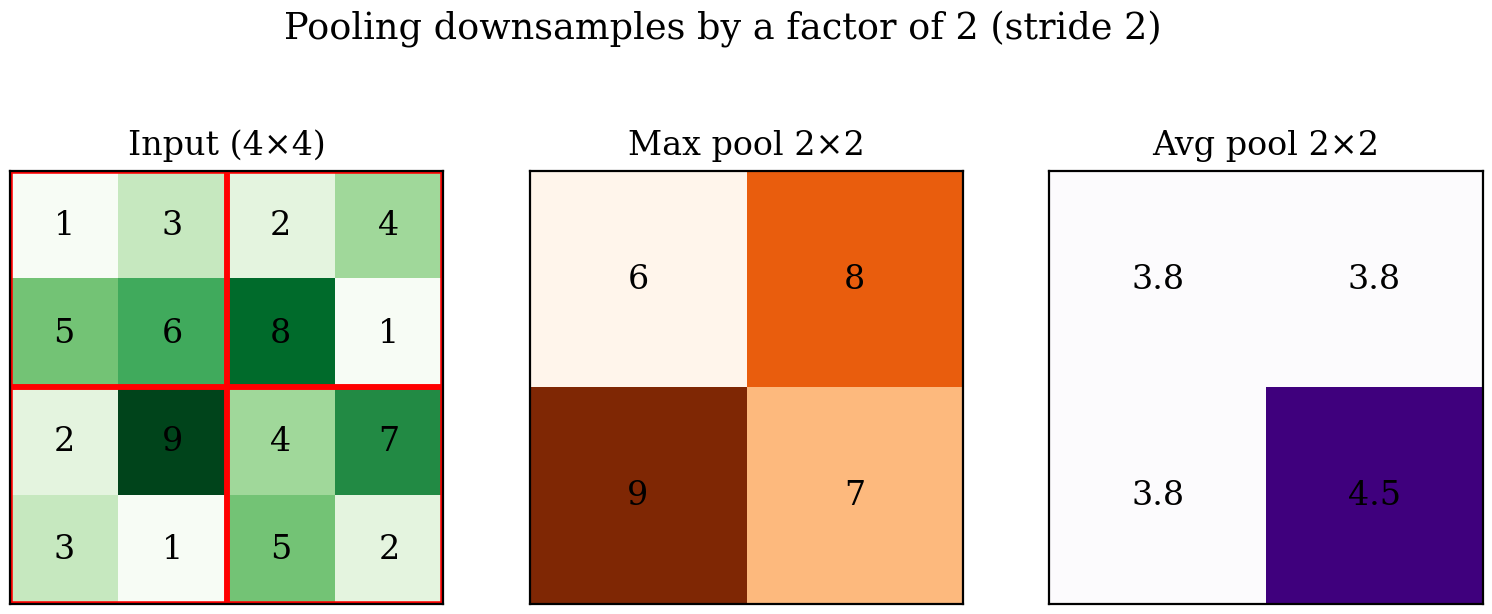
\includegraphics[width=0.92\linewidth]{figures/pooling.png}
\caption{Max vs average pooling with a $2\times2$ window and stride 2. Both halve
each spatial dimension; max pooling keeps the dominant response, average pooling
the local mean.}
\label{fig:pool}
\end{figure}

\section{Activation functions}

Without a non-linearity, a stack of convolutions collapses to a single linear
map. The activation $\phi$ applied element-wise after each layer gives the
network its expressive power (Figure~\ref{fig:act}). The default is the
rectified linear unit:
\begin{equation}
\mathrm{ReLU}(z)=\max(0,z).
\end{equation}
ReLU is cheap, non-saturating for $z>0$, and induces sparsity, but ``dead''
units can occur when a neuron is pushed permanently negative.
\emph{LeakyReLU}, $\phi(z)=\max(\alpha z,z)$ with small $\alpha$, keeps a
gradient for $z<0$. \emph{GELU}, $\phi(z)=z\,\Phi(z)$ (with $\Phi$ the Gaussian
CDF), is a smooth variant favoured in transformers. The saturating
\emph{sigmoid} $\sigma(z)=1/(1+e^{-z})$ and \emph{tanh} are now used mainly in
output layers (binary probability) or gates, because their vanishing gradients
slow deep training.

\begin{figure}[h]
\centering
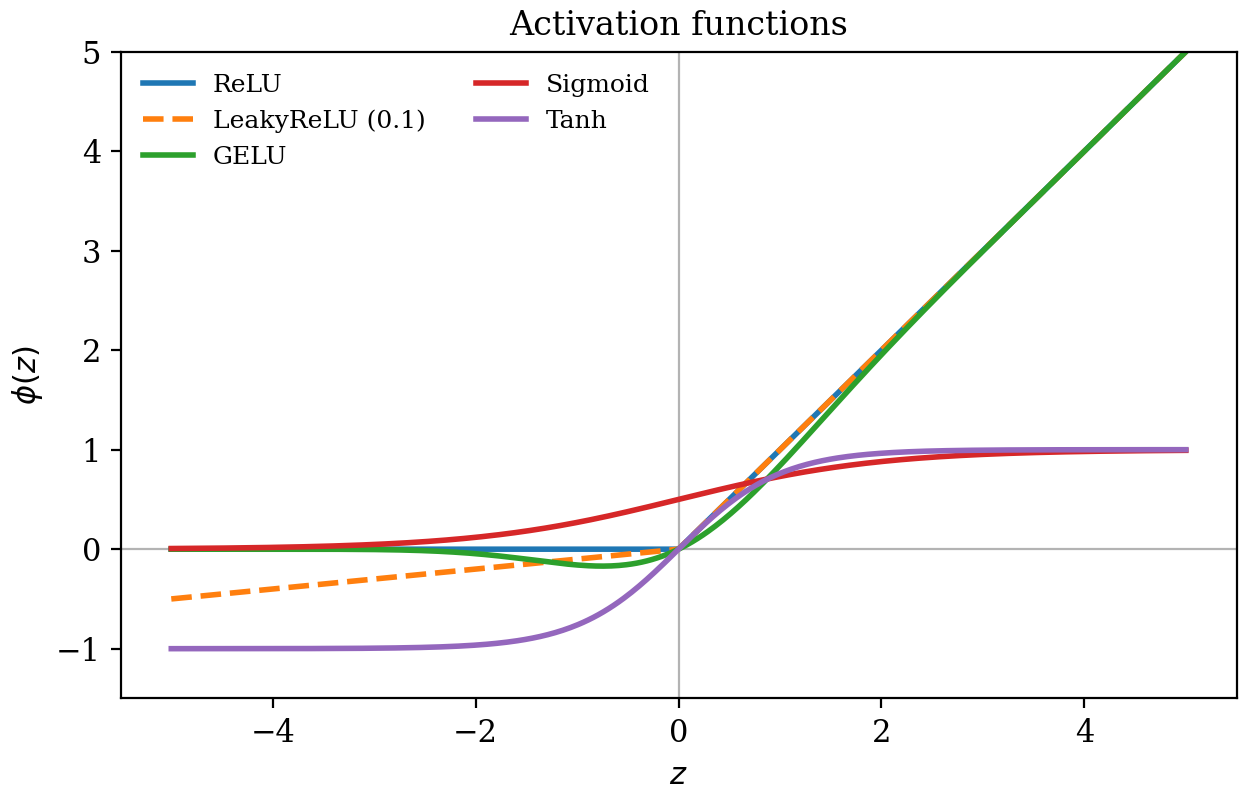
\includegraphics[width=0.68\linewidth]{figures/activations.png}
\caption{Common activation functions. ReLU and its smooth relatives (LeakyReLU,
GELU) dominate hidden layers; sigmoid/tanh saturate and are reserved for outputs
and gates.}
\label{fig:act}
\end{figure}

\section{Batch normalisation}

Batch normalisation (Ioffe \& Szegedy, 2015) normalises each channel's
pre-activations across the mini-batch, then rescales with learnable parameters
$\gamma,\beta$. For a channel with batch values $\{x_i\}$:
\begin{align}
\mu_B &= \frac1m\sum_i x_i, &
\sigma_B^2 &= \frac1m\sum_i (x_i-\mu_B)^2,\\
\hat x_i &= \frac{x_i-\mu_B}{\sqrt{\sigma_B^2+\epsilon}}, &
y_i &= \gamma\,\hat x_i + \beta.
\label{eq:bn}
\end{align}
BatchNorm reduces \emph{internal covariate shift}, smooths the loss landscape,
permits higher learning rates, and acts as a mild regulariser. At inference it
uses running estimates of $\mu,\sigma$ accumulated during training. Because BN
already provides a per-channel shift $\beta$, the preceding convolution sets
\texttt{bias=False}. Place it as \texttt{Conv $\to$ BN $\to$ ReLU}.

\begin{notebox}[Small-batch caveat]
BatchNorm statistics are unreliable with very small batches (common for
high-resolution segmentation on limited VRAM). In that regime prefer GroupNorm
or InstanceNorm, which normalise without a batch dependency.
\end{notebox}

\section{Dropout and overfitting}

Overfitting occurs when a model memorises training data and fails to generalise;
its signature is a training loss that keeps falling while validation loss rises.
\emph{Dropout} (Srivastava et al., 2014) combats this by randomly zeroing a
fraction $p$ of activations during training, scaling the survivors by
$1/(1-p)$, which prevents co-adaptation and approximates an ensemble. It is
disabled at inference. In convolutional bodies dropout is used sparingly
(spatial structure makes element-wise dropout weak); it is most effective in
the dense head. The stronger regularisers for CNNs are data augmentation
(Chapter~\ref{ch:aug}), weight decay, and BatchNorm itself.

\section{Assembling a CNN}

A canonical small classifier stacks \emph{blocks} of
\texttt{Conv$\to$BN$\to$ReLU$\to$Pool}, doubling channels as resolution halves,
then a GAP and a linear classifier:
\begin{lstlisting}
import torch.nn as nn
class ConvBlock(nn.Module):
    def __init__(self, cin, cout):
        super().__init__()
        self.net = nn.Sequential(
            nn.Conv2d(cin, cout, 3, padding=1, bias=False),
            nn.BatchNorm2d(cout), nn.ReLU(inplace=True),
            nn.MaxPool2d(2))            # halves H, W
    def forward(self, x): return self.net(x)

class SimpleCNN(nn.Module):
    def __init__(self, in_ch=3, n_classes=10):
        super().__init__()
        self.features = nn.Sequential(
            ConvBlock(in_ch, 32),       # 64 -> 32
            ConvBlock(32, 64),          # 32 -> 16
            ConvBlock(64, 128))         # 16 -> 8
        self.head = nn.Sequential(
            nn.AdaptiveAvgPool2d(1), nn.Flatten(),
            nn.Dropout(0.3), nn.Linear(128, n_classes))
    def forward(self, x): return self.head(self.features(x))
\end{lstlisting}
The channel-doubling/resolution-halving rule keeps the per-layer compute roughly
constant while building an increasingly abstract, lower-resolution
representation --- a pattern you will see again in every ResNet and U-Net
encoder.

\begin{keybox}
\begin{itemize}[leftmargin=1.2em,nosep]
  \item Pooling/strides downsample and grow the RF; GAP replaces heavy FC heads.
  \item ReLU is the default hidden activation; sigmoid/tanh for outputs/gates.
  \item BatchNorm (Eq.~\ref{eq:bn}) stabilises and speeds training; order is Conv$\to$BN$\to$ReLU, bias off.
  \item Overfitting $=$ train loss $\downarrow$ while val loss $\uparrow$; fight it with augmentation, weight decay, dropout.
  \item Standard pattern: blocks of Conv-BN-ReLU-Pool, doubling channels, then GAP + linear.
\end{itemize}
\end{keybox}

\begin{practbox}
Notebook: \nbpath{chapter\_03\_cnn\_building\_blocks/03\_practical\_cnn\_components.ipynb}.
\begin{enumerate}[leftmargin=1.4em,nosep]
  \item Visually compare max vs average pooling on a sample feature map.
  \item Plot ReLU, LeakyReLU, GELU, sigmoid and tanh and their gradients.
  \item Train a small net \emph{with} and \emph{without} BatchNorm; compare loss
  curves and the largest stable learning rate.
  \item Force overfitting on a tiny subset, then add dropout and observe the
  validation-loss gap shrink.
  \item Build \texttt{SimpleCNN}; print a layer-by-layer summary of shapes and
  parameter counts.
\end{enumerate}
\end{practbox}

\begin{exbox}
\textbf{3.1 Architecture ablation.} Vary depth (2 vs 3 vs 4 blocks) and width
(16/32/64 base channels); tabulate parameters, train time and accuracy.\\[2pt]
\textbf{3.2 Normalisation swap.} Replace BatchNorm with GroupNorm; retrain at
batch size 4 and explain the difference.\\[2pt]
\textbf{3.3 Activation study.} Swap ReLU for LeakyReLU and GELU; measure
convergence speed and final accuracy.\\[2pt]
\textbf{Mini-project.} Implement a configurable \texttt{make\_cnn(depth, width,
norm, act, dropout)} factory and run a small grid search on EuroSAT, reporting a
parameters-vs-accuracy scatter plot.
\end{exbox}

\chapter{Remote Sensing Data and Geospatial Preprocessing}
\label{ch:preproc}

\chapmeta{Beginner $\to$ Intermediate}{$\sim$5\,h (2.5\,h + 2.5\,h)}{Sentinel-2 sample tiles; synthetic scenes}

\begin{objbox}
\begin{itemize}[leftmargin=1.2em,nosep]
  \item Read and write multi-band GeoTIFFs with \texttt{rasterio} and \texttt{rioxarray}.
  \item Understand CRS, geotransforms, and band resolution mismatches.
  \item Compute spectral indices (NDVI, NDWI, NDBI, EVI) as engineered channels.
  \item Choose and apply a normalization strategy for reflectance data.
  \item Tile a large scene into model-ready patches and reconstruct it.
\end{itemize}
\end{objbox}

This is the first genuinely Earth-Observation chapter: turning a raw
multispectral scene into tensors a CNN can train on. The steps --- loading,
index computation, normalization, tiling --- form the front half of every
pipeline in the rest of the book.

\section{Reading multi-band rasters}

A GeoTIFF couples a pixel grid with georeferencing: a CRS and an affine
\emph{geotransform} mapping array indices to world coordinates,
\begin{equation}
\begin{pmatrix}x\\y\end{pmatrix}
=\begin{pmatrix}a & b\\ d & e\end{pmatrix}\!\begin{pmatrix}\mathrm{col}\\ \mathrm{row}\end{pmatrix}
+\begin{pmatrix}c\\ f\end{pmatrix},
\end{equation}
where $(c,f)$ is the top-left corner and $a,e$ are the pixel sizes (with
$e<0$). \texttt{rasterio} exposes this as \texttt{src.transform} and the
projection as \texttt{src.crs}.
\begin{lstlisting}
import rasterio
with rasterio.open("scene.tif") as src:
    arr = src.read()          # (bands, H, W), native dtype (uint16 reflectance)
    profile = src.profile      # crs, transform, dtype, nodata, ...
\end{lstlisting}
\texttt{rioxarray} wraps the same data as a labelled \texttt{xarray.DataArray}
with named dimensions and coordinates, which is convenient for band maths and
resampling. A practical complication is that Sentinel-2 bands have \emph{mixed
resolutions} (10/20/60\,m); to stack them into one tensor you resample the
20/60\,m bands to the 10\,m grid (bilinear for continuous reflectance).

\section{Spectral indices as engineered features}

Normalised-difference indices are cheap, physically motivated channels that
often boost segmentation accuracy on the classes they target:
\begin{align}
\mathrm{NDVI} &= \frac{\mathrm{B08}-\mathrm{B04}}{\mathrm{B08}+\mathrm{B04}} &&\text{(vegetation)},\\
\mathrm{NDWI} &= \frac{\mathrm{B03}-\mathrm{B08}}{\mathrm{B03}+\mathrm{B08}} &&\text{(open water)},\\
\mathrm{NDBI} &= \frac{\mathrm{B11}-\mathrm{B08}}{\mathrm{B11}+\mathrm{B08}} &&\text{(built-up)},\\
\mathrm{EVI} &= 2.5\,\frac{\mathrm{B08}-\mathrm{B04}}{\mathrm{B08}+6\,\mathrm{B04}-7.5\,\mathrm{B02}+1} &&\text{(canopy, haze-robust)}.
\end{align}
Figure~\ref{fig:ndvi} shows a synthetic scene and its NDVI: forest and crops
light up, water goes negative. Appending such indices as extra channels gives
the network features it might otherwise have to learn from scratch.

\begin{figure}[h]
\centering
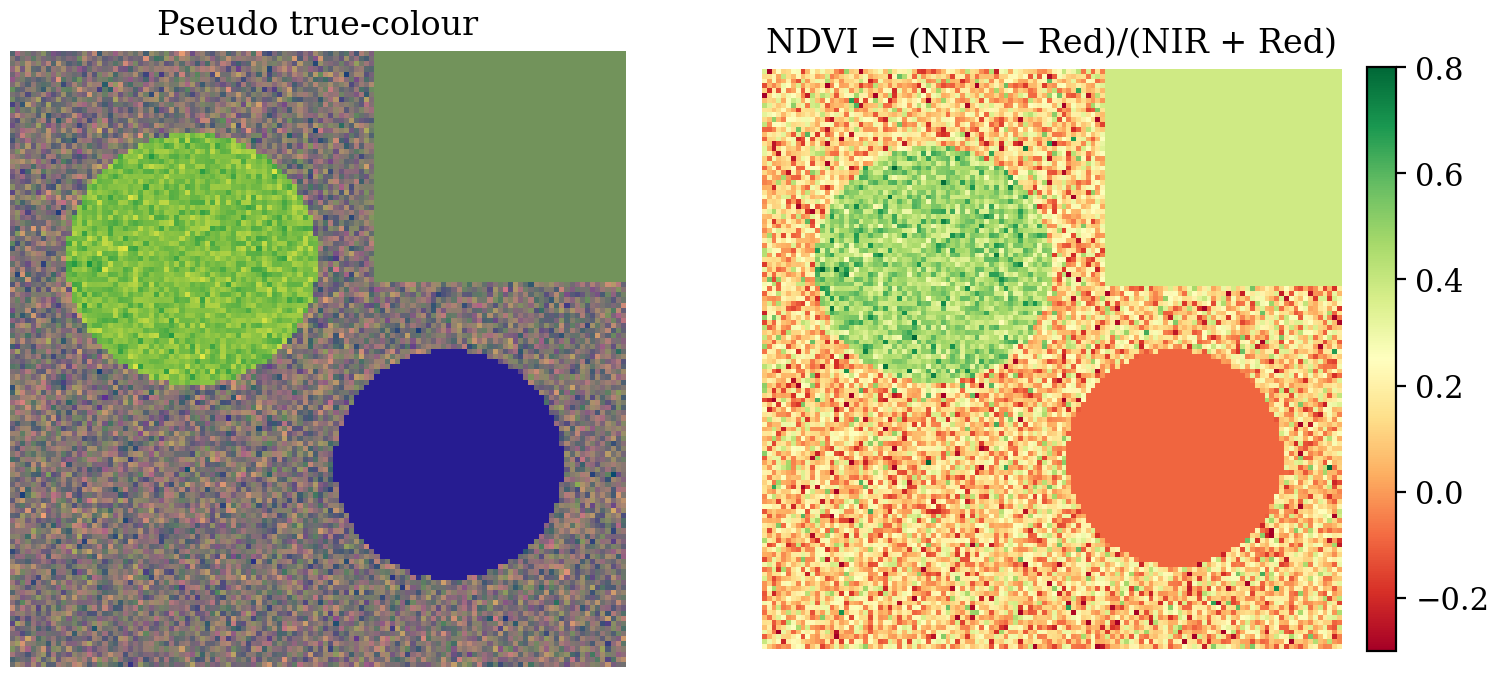
\includegraphics[width=0.86\linewidth]{figures/ndvi.png}
\caption{A pseudo true-colour scene (left) and its NDVI (right). High NDVI
(green) marks vegetation; water is strongly negative (red). Indices encode
domain knowledge as ready-made input channels.}
\label{fig:ndvi}
\end{figure}

\section{Normalization strategies}

Networks train best on inputs with comparable, $O(1)$ scales. Raw Sentinel-2
digital numbers span $0$--$10000$ and differ per band, so normalization is
mandatory (Figure~\ref{fig:norm}). Three common strategies:
\begin{description}[leftmargin=1.5em,style=nextline]
  \item[Min--max] $x'=(x-x_{\min})/(x_{\max}-x_{\min})\in[0,1]$. Simple but
  sensitive to outliers (a single bright cloud rescales everything).
  \item[Percentile clip] map the 2nd--98th percentile to $[0,1]$ and clip. Robust
  to outliers; the standard for visualisation and a strong default for training.
  \item[Z-score] $x'=(x-\mu_c)/\sigma_c$ with \emph{per-band} dataset statistics
  $\mu_c,\sigma_c$. Pairs naturally with ImageNet-pretrained encoders (which
  expect standardised inputs).
\end{description}

\begin{figure}[h]
\centering
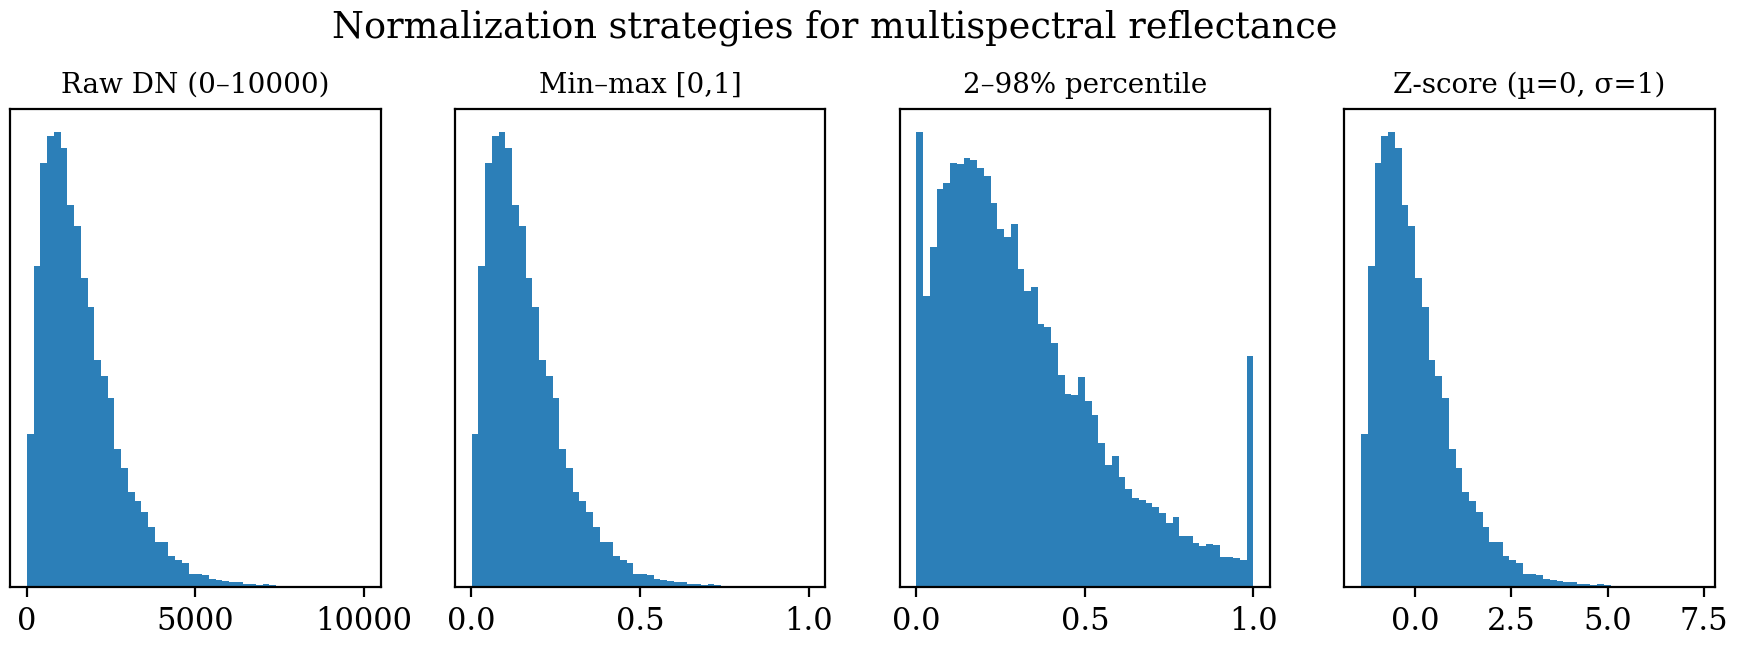
\includegraphics[width=\linewidth]{figures/normalization.png}
\caption{Effect of normalization on a reflectance histogram. Percentile clipping
tames the long bright tail; z-scoring centres each band at zero with unit
variance --- the form pretrained encoders expect.}
\label{fig:norm}
\end{figure}

\begin{notebox}[Train/serve consistency]
Compute normalization statistics on the \emph{training} set only and reuse them
unchanged for validation, test and inference. Recomputing per-image or per-split
statistics leaks information and breaks reproducibility in the deployed pipeline.
\end{notebox}

\section{Tiling a scene}

Sentinel-2 tiles are $\sim$$10980\times10980$ pixels --- far too large for a GPU.
We cut them into fixed patches (e.g.\ $512\times512$) with an overlap so that the
later sliding-window inference (Chapter~\ref{ch:pipeline}) can blend predictions
and avoid seams. Given tile size $T$ and stride $s<T$ (overlap $T-s$), tile
origins are $\{(i s, j s)\}$ clipped to the scene; edge tiles are padded.
Reconstruction reverses the process, accumulating predictions and dividing by a
weight map. A reusable preprocessing class typically chains: load $\to$ resample
$\to$ compute indices $\to$ normalize $\to$ tile, returning $(C,T,T)$ tensors
plus each tile's geotransform for georeferenced export later.

\begin{keybox}
\begin{itemize}[leftmargin=1.2em,nosep]
  \item GeoTIFF $=$ pixels $+$ CRS $+$ affine geotransform; read with \texttt{rasterio}/\texttt{rioxarray}.
  \item Resample mixed-resolution bands to a common grid before stacking.
  \item Spectral indices (NDVI/NDWI/NDBI/EVI) are cheap, informative extra channels.
  \item Normalize (percentile clip or per-band z-score) using \emph{training} statistics only.
  \item Tile large scenes with overlap; keep each tile's transform for export.
\end{itemize}
\end{keybox}

\begin{practbox}
Notebook: \nbpath{chapter\_04\_geospatial\_preprocessing/04\_practical\_sentinel2\_preprocessing.ipynb}.
\begin{enumerate}[leftmargin=1.4em,nosep]
  \item Generate (or download) a synthetic multi-band Sentinel-2 GeoTIFF; inspect
  shape, CRS, transform and per-band ranges with \texttt{rasterio}.
  \item Render true-colour and false-colour (NIR-Red-Green) composites.
  \item Load with \texttt{rioxarray}; compute NDVI and NDWI as new DataArrays.
  \item Compare min--max, percentile and z-score normalization via histograms.
  \item Implement \texttt{tile\_scene} / \texttt{reconstruct\_from\_tiles} and
  verify a round-trip reconstructs the input exactly.
\end{enumerate}
\begin{lstlisting}
def percentile_norm(band, lo=2, hi=98):
    p_lo, p_hi = np.percentile(band, [lo, hi])
    return np.clip((band - p_lo) / (p_hi - p_lo + 1e-6), 0, 1)
\end{lstlisting}
\end{practbox}

\begin{exbox}
\textbf{4.1 Real data.} Download a real Sentinel-2 L2A tile (e.g.\ via the
Copernicus browser or \texttt{sentinelsat}); load four 10\,m bands and resample
two 20\,m bands to 10\,m.\\[2pt]
\textbf{4.2 Index zoo.} Implement NDVI, NDWI, NDBI and EVI as functions; display
each over a real scene and interpret the highlighted land cover.\\[2pt]
\textbf{4.3 Overlap study.} Tile a scene at 0\%, 25\% and 50\% overlap; count
tiles and discuss the inference cost/quality trade-off.\\[2pt]
\textbf{Mini-project.} Build a \texttt{Sentinel2Tile} class that loads bands,
appends two indices, percentile-normalizes, and yields georeferenced
$512\times512$ tiles ready for a \texttt{DataLoader}.
\end{exbox}


\part{Classification: The First Complete Pipeline}
\chapter{The First Complete Classification Pipeline}
\label{ch:classif}

\chapmeta{Intermediate}{$\sim$5\,h (2\,h + 3\,h)}{EuroSAT (torchgeo)}

\begin{objbox}
\begin{itemize}[leftmargin=1.2em,nosep]
  \item Derive softmax and the cross-entropy loss for multi-class classification.
  \item Build train/validation/test \texttt{DataLoader}s from a \texttt{torchgeo} dataset.
  \item Write a complete training loop with validation, checkpointing and metrics.
  \item Diagnose training from loss/accuracy curves.
  \item Evaluate on a held-out test set and interpret the result.
\end{itemize}
\end{objbox}

We now assemble the building blocks of Chapter~\ref{ch:blocks} into an
end-to-end pipeline that trains \texttt{SimpleCNN} to classify EuroSAT patches.
This is the template every later pipeline reuses --- only the data, model and
loss change.

\section{Softmax and cross-entropy}

A classifier outputs a vector of \emph{logits} $\mathbf{z}\in\R^{K}$ (one per
class). The softmax turns logits into a probability distribution:
\begin{equation}
p_k = \mathrm{softmax}(\mathbf{z})_k = \frac{e^{z_k}}{\sum_{j=1}^{K} e^{z_j}},
\qquad \sum_k p_k = 1.
\end{equation}
For a sample with true class $y$, the (categorical) cross-entropy loss is the
negative log-likelihood of the correct class:
\begin{equation}
\mathcal{L}_{\mathrm{CE}} = -\log p_y = -z_y + \log\sum_{j} e^{z_j}.
\label{eq:ce}
\end{equation}
Its gradient with respect to the logits is strikingly simple,
\begin{equation}
\frac{\partial \mathcal{L}_{\mathrm{CE}}}{\partial z_k} = p_k - \mathbb{1}[k=y],
\end{equation}
i.e.\ ``predicted minus target''. The loss explodes when the model is
confidently wrong ($p_y\to 0$) and vanishes when confidently right
(Figure~\ref{fig:ce}). In PyTorch, \texttt{nn.CrossEntropyLoss} fuses
log-softmax and NLL for numerical stability and expects \emph{raw logits} ---
never apply softmax before it.

\begin{figure}[h]
\centering
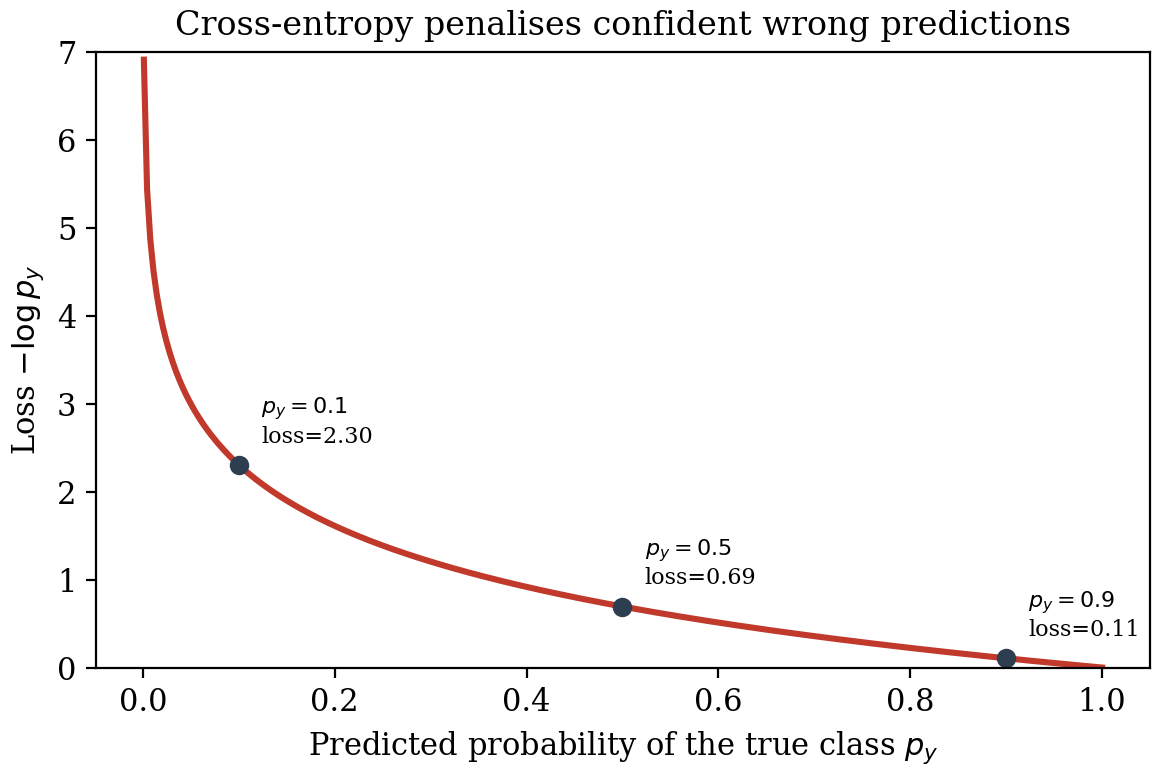
\includegraphics[width=0.6\linewidth]{figures/crossentropy.png}
\caption{Cross-entropy as a function of the predicted probability of the true
class. The steep penalty near $p_y=0$ is what drives the network to be both
correct and calibrated.}
\label{fig:ce}
\end{figure}

\section{Data loading with torchgeo}

\texttt{torchgeo} downloads EuroSAT and yields samples as dictionaries
(\texttt{\{"image":\dots,"label":\dots\}}), so we provide a small
\texttt{collate\_fn} and wrap splits in \texttt{DataLoader}s. We normalize with
the per-channel statistics computed in Chapter~\ref{ch:intro} and shuffle only
the training split.
\begin{lstlisting}
from torch.utils.data import DataLoader, random_split
def collate(batch):
    imgs = torch.stack([b["image"].float()/3000. for b in batch])
    lbls = torch.tensor([int(b["label"]) for b in batch])
    return imgs, lbls
train_dl = DataLoader(train_ds, batch_size=64, shuffle=True,
                      num_workers=2, collate_fn=collate)
\end{lstlisting}
A correct split is non-negotiable: the test set is touched \emph{once}, at the
very end. Use a fixed seed so splits are reproducible.

\section{The training loop}

One epoch iterates the training loader, and for each batch performs the five
canonical steps: forward, loss, backward, step, zero-grad. After each epoch we
evaluate on the validation set (no gradients) and checkpoint the best model.
\begin{lstlisting}
import torch
opt = torch.optim.AdamW(model.parameters(), lr=1e-3, weight_decay=1e-4)
crit = torch.nn.CrossEntropyLoss()
for epoch in range(EPOCHS):
    model.train()
    for x, y in train_dl:
        x, y = x.to(DEVICE), y.to(DEVICE)
        opt.zero_grad()
        loss = crit(model(x), y)
        loss.backward()
        torch.nn.utils.clip_grad_norm_(model.parameters(), 5.0)
        opt.step()
    val_acc = evaluate(model, val_dl)        # no_grad, argmax == y
    if val_acc > best: torch.save(model.state_dict(), "best.pth")
\end{lstlisting}
Several details matter in practice: \texttt{model.train()}/\texttt{model.eval()}
toggle BatchNorm and dropout; \texttt{torch.no\_grad()} during validation saves
memory; gradient clipping guards against rare exploding updates; and AdamW's
decoupled weight decay regularises. A learning-rate scheduler (cosine or
step) usually adds a point or two of accuracy.

\section{Reading the curves}

Plot training and validation loss and accuracy every epoch
(Figure~\ref{fig:curves}). A healthy run shows both losses descending and then
plateauing close together. A growing gap --- validation loss rising while
training loss falls --- signals overfitting and calls for more augmentation
(Chapter~\ref{ch:aug}), weight decay, or early stopping. A validation loss that
never descends usually means a too-small/too-large learning rate or a data
bug (e.g.\ unnormalised inputs, wrong label mapping).

\begin{figure}[h]
\centering
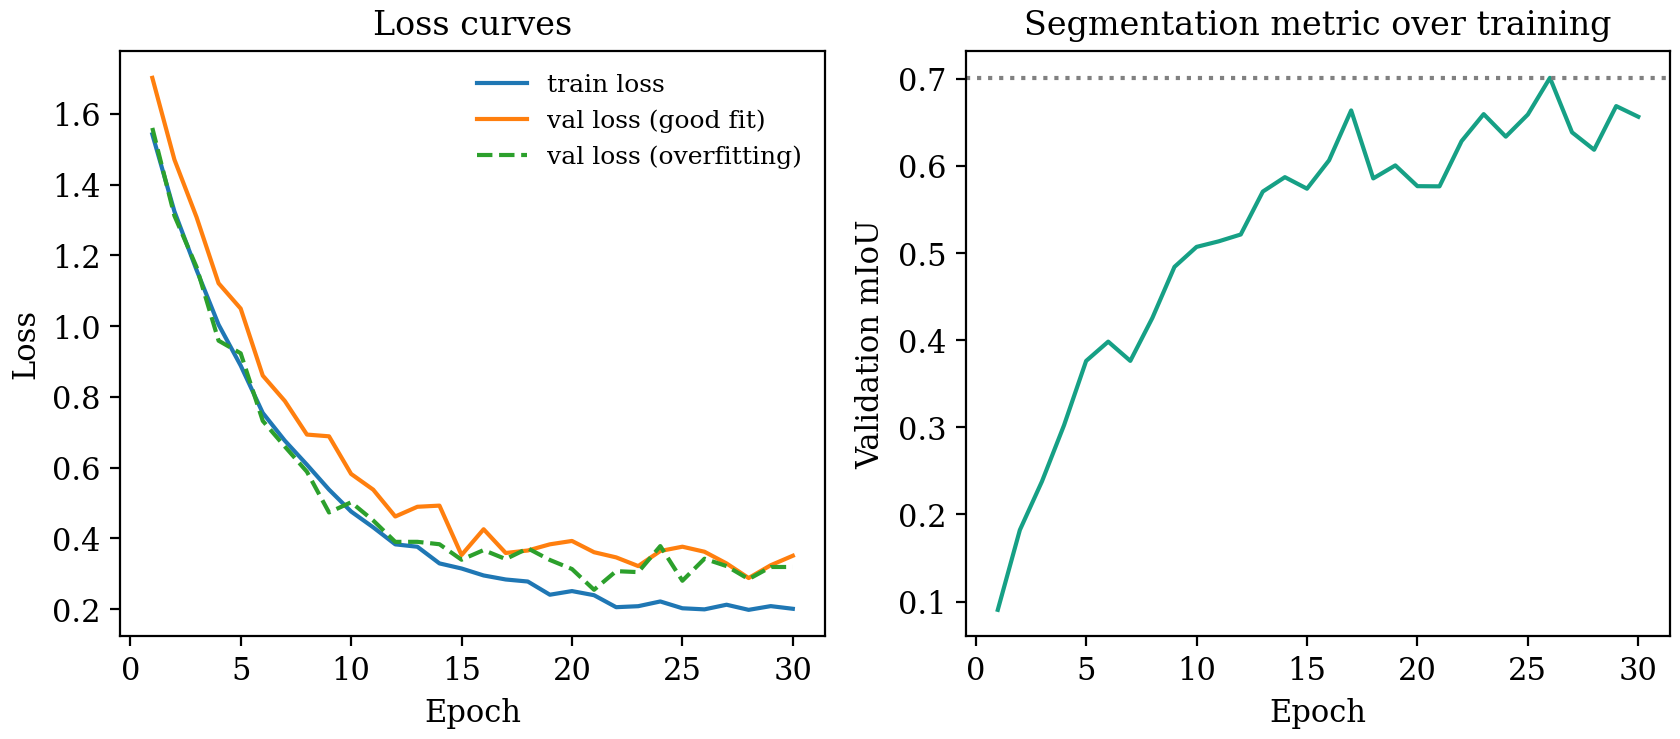
\includegraphics[width=0.95\linewidth]{figures/training_curves.png}
\caption{Left: loss curves. The dashed curve diverging upward is the classic
overfitting signature. Right: a validation metric (here mIoU) saturating ---
the best epoch (dotted line) is the one to checkpoint.}
\label{fig:curves}
\end{figure}

\section{Final evaluation}

Reload the best checkpoint and evaluate \emph{once} on the test set. Report
overall accuracy and the per-class confusion matrix (Chapter~\ref{ch:eval}); a
well-trained \texttt{SimpleCNN} reaches the high-80s/low-90s on EuroSAT RGB,
while a fine-tuned ResNet (Chapters~\ref{ch:arch}--\ref{ch:transfer}) exceeds
98\%. Confusions cluster among spectrally similar classes (e.g.\ \textsf{AnnualCrop}
vs \textsf{PermanentCrop}), a hint that spatial context and more bands help.

\begin{keybox}
\begin{itemize}[leftmargin=1.2em,nosep]
  \item Softmax $\to$ probabilities; cross-entropy (Eq.~\ref{eq:ce}) is NLL of the true class; feed \emph{logits} to \texttt{CrossEntropyLoss}.
  \item Five-step loop: forward, loss, backward, step, zero-grad; toggle \texttt{train()}/\texttt{eval()}.
  \item Checkpoint on best validation metric; touch the test set only once.
  \item Diverging val loss $=$ overfitting; flat val loss $=$ LR or data bug.
\end{itemize}
\end{keybox}

\begin{practbox}
Notebook: \nbpath{chapter\_05\_classification\_pipeline/05\_practical\_eurosat\_classification.ipynb}.
\begin{enumerate}[leftmargin=1.4em,nosep]
  \item Visualise cross-entropy behaviour for varying $p_y$.
  \item Build EuroSAT loaders with a custom \texttt{collate\_fn} and normalization.
  \item Train \texttt{SimpleCNN} for $\sim$15 epochs with AdamW + cosine schedule.
  \item Plot loss/accuracy curves; identify the best epoch.
  \item Load the best checkpoint, evaluate on test, print accuracy and confusion matrix.
\end{enumerate}
\end{practbox}

\begin{exbox}
\textbf{5.1 LR sensitivity.} Sweep learning rates $\{10^{-2},10^{-3},10^{-4}\}$;
plot final accuracy and discuss the U-shape.\\[2pt]
\textbf{5.2 Class weighting.} Add \texttt{weight=} to \texttt{CrossEntropyLoss}
using inverse class frequency; measure the effect on the weakest class.\\[2pt]
\textbf{5.3 Early stopping.} Implement patience-based early stopping; compare the
selected epoch with the full-run best.\\[2pt]
\textbf{Mini-project.} Wrap everything into a reusable \texttt{ClassificationTrainer}
with history logging, checkpointing and early stopping; reproduce your manual
result through the class API.
\end{exbox}

\chapter{CNN Architectures: VGG, ResNet, EfficientNet}
\label{ch:arch}

\chapmeta{Intermediate}{$\sim$4\,h (2\,h + 2\,h)}{EuroSAT}

\begin{objbox}
\begin{itemize}[leftmargin=1.2em,nosep]
  \item Trace the evolution from LeNet/AlexNet/VGG to ResNet and EfficientNet.
  \item Explain the degradation problem and how residual connections solve it.
  \item Implement a ResNet basic block and reason about gradient flow.
  \item Understand EfficientNet's compound scaling and the accuracy/efficiency frontier.
  \item Swap backbones in a classifier and compare parameters, speed and accuracy.
\end{itemize}
\end{objbox}

\section{A short architectural history}

LeNet-5 (1998) established the \texttt{conv--pool--FC} template. AlexNet (2012)
scaled it up with ReLU, dropout and GPU training, winning ImageNet by a wide
margin. VGG (2014) showed that \emph{depth} built from uniform $3\times3$
convolutions works well --- recall (Chapter~\ref{ch:conv}) that two stacked
$3\times3$ layers match a $5\times5$ receptive field with fewer parameters and
an extra non-linearity. But naively stacking ever more layers \emph{degraded}
accuracy, even on the training set --- not overfitting, but an optimisation
failure. ResNet (2015) fixed this and remains the default EO encoder.

\section{The degradation problem and residual connections}

A residual block learns a \emph{residual} $\mathcal{F}(\mathbf{x})$ added to its
input via a skip (identity) connection:
\begin{equation}
\mathbf{y} = \mathcal{F}(\mathbf{x}; \{W_i\}) + \mathbf{x}.
\label{eq:resid}
\end{equation}
If the optimal mapping for a block is close to the identity, it is far easier to
drive $\mathcal{F}\to 0$ than to make a stack of nonlinear layers represent the
identity exactly. Crucially, the skip provides a gradient highway: by the chain
rule the gradient reaching $\mathbf{x}$ contains an additive ``$+1$'' term,
\begin{equation}
\frac{\partial \mathcal{L}}{\partial \mathbf{x}}
= \frac{\partial \mathcal{L}}{\partial \mathbf{y}}
\left(1 + \frac{\partial \mathcal{F}}{\partial \mathbf{x}}\right),
\end{equation}
so gradients cannot vanish merely from depth. This lets networks train at 50,
101, even 152 layers. Figure~\ref{fig:resblock} shows the basic block.

\begin{figure}[h]
\centering
\fitwidth{
\begin{tikzpicture}[font=\small,>=Latex,node distance=8mm]
  \tikzstyle{op}=[draw,rounded corners,minimum width=26mm,minimum height=7mm,fill=eoblue!8]
  \node (x) {$\mathbf{x}$};
  \node[op,right=8mm of x] (c1) {Conv $3\times3$};
  \node[op,right=6mm of c1] (b1) {BN};
  \node[op,right=6mm of b1] (r1) {ReLU};
  \node[op,right=6mm of r1] (c2) {Conv $3\times3$};
  \node[op,right=6mm of c2] (b2) {BN};
  \node[draw,circle,right=10mm of b2,inner sep=1.5pt] (sum) {$+$};
  \node[op,right=8mm of sum,fill=eogreen!12] (r2) {ReLU};
  \node[right=8mm of r2] (y) {$\mathbf{y}$};
  \draw[->] (x)--(c1); \draw[->] (c1)--(b1); \draw[->] (b1)--(r1);
  \draw[->] (r1)--(c2); \draw[->] (c2)--(b2); \draw[->] (b2)--(sum);
  \draw[->] (sum)--(r2); \draw[->] (r2)--(y);
  \draw[->,eored,thick] (x.south) -- ++(0,-9mm) -| (sum.south)
        node[pos=0.25,below,black]{identity skip $\mathbf{x}$};
\end{tikzpicture}}
\caption{ResNet basic block (Eq.~\ref{eq:resid}). The identity skip (red) lets
the block default to a near-identity map and gives gradients an unobstructed
path, enabling very deep training. A $1\times1$ ``projection'' conv replaces the
skip when channel count or resolution changes.}
\label{fig:resblock}
\end{figure}

Deeper ResNets replace the two-$3\times3$ block with a \emph{bottleneck}
($1\times1\to3\times3\to1\times1$) that reduces and then restores channel
dimension, cutting cost while keeping capacity --- the building block of
ResNet-50/101.

\section{EfficientNet and compound scaling}

Networks can grow along three axes: depth (layers), width (channels) and input
resolution. EfficientNet (2019) showed these should be scaled \emph{together} in
fixed ratios governed by a single compound coefficient $\phi$:
\begin{equation}
\text{depth} \propto \alpha^{\phi},\quad
\text{width} \propto \beta^{\phi},\quad
\text{resolution} \propto \gamma^{\phi},\qquad
\alpha\beta^2\gamma^2 \approx 2,
\end{equation}
where increasing $\phi$ by one roughly doubles compute. Built on
mobile inverted-bottleneck (MBConv) blocks with squeeze-and-excitation,
EfficientNet-B0$\dots$B7 trace an accuracy/efficiency frontier that beats
ResNets at equal FLOPs --- attractive when EO inference must run cheaply at
scale.

\section{Swapping backbones}

In code, changing architecture is a one-line change because \texttt{torchvision}
and \texttt{timm} expose a uniform API:
\begin{lstlisting}
import torchvision.models as tv
m18 = tv.resnet18(weights=None, num_classes=10)
m50 = tv.resnet50(weights=None, num_classes=10)
import timm
eff = timm.create_model("efficientnet_b0", num_classes=10, in_chans=3)
\end{lstlisting}
Benchmarking on EuroSAT typically shows ResNet18 ($\sim$11\,M params) training
fastest, ResNet50 ($\sim$25\,M) slightly more accurate, and EfficientNet-B0
($\sim$5\,M) matching ResNet50 accuracy at a fraction of the parameters --- the
point of compound scaling. The same encoders reappear inside segmentation
decoders in Chapters~\ref{ch:seg}--\ref{ch:advseg}, which is exactly why we study
them now.

\begin{keybox}
\begin{itemize}[leftmargin=1.2em,nosep]
  \item VGG: depth from stacked $3\times3$; expensive FC head.
  \item Degradation $\ne$ overfitting; residual skips (Eq.~\ref{eq:resid}) solve it and ease gradient flow.
  \item Bottleneck blocks scale ResNet to 50/101/152 layers efficiently.
  \item EfficientNet scales depth/width/resolution jointly; best accuracy per FLOP.
  \item The classification encoder is reused as the segmentation encoder later.
\end{itemize}
\end{keybox}

\begin{practbox}
Notebook: \nbpath{chapter\_06\_cnn\_architectures/06\_practical\_cnn\_architectures.ipynb}.
\begin{enumerate}[leftmargin=1.4em,nosep]
  \item Implement a \texttt{BasicBlock} from scratch with the identity skip.
  \item Visualise gradient magnitude per layer \emph{with} and \emph{without} the
  skip to see the gradient highway.
  \item Tabulate parameters, forward-pass latency and accuracy for ResNet18/50 and
  EfficientNet-B0.
  \item Train ResNet18 vs EfficientNet-B0 on EuroSAT for a few epochs and compare.
\end{enumerate}
\end{practbox}

\begin{exbox}
\textbf{6.1 Bottleneck block.} Implement the $1\times1\to3\times3\to1\times1$
bottleneck and verify the parameter saving versus two $3\times3$ layers at equal
channels.\\[2pt]
\textbf{6.2 Depth ablation.} Build plain (no-skip) vs residual nets of increasing
depth; show that only the residual ones keep improving.\\[2pt]
\textbf{6.3 Width vs depth.} At a fixed parameter budget, compare a wider-shallow
and a narrower-deep network on EuroSAT.\\[2pt]
\textbf{Mini-project.} Write \texttt{build\_classifier(backbone, n\_classes)}
supporting ResNet18/50 and EfficientNet-B0, and a benchmark harness that outputs
a params-vs-accuracy plot.
\end{exbox}

\chapter{Transfer Learning for Earth Observation}
\label{ch:transfer}

\chapmeta{Intermediate}{$\sim$5\,h (2\,h + 3\,h)}{EuroSAT RGB + MS}

\begin{objbox}
\begin{itemize}[leftmargin=1.2em,nosep]
  \item Explain why ImageNet features transfer to satellite imagery --- and their limits.
  \item Distinguish the three transfer regimes: feature extraction, fine-tuning, from scratch.
  \item Adapt an RGB-pretrained first convolution to multispectral input.
  \item Apply discriminative (layer-wise) learning rates and progressive unfreezing.
  \item Quantify the accuracy and data-efficiency gains from pretraining.
\end{itemize}
\end{objbox}

\section{Why ImageNet transfers to EO}

A network pretrained on ImageNet has already learned, in its early layers, a
generic visual vocabulary: oriented edges, colour-opponent filters, blobs and
textures. These low- and mid-level features are \emph{not} specific to cats and
cars --- they describe natural images in general, and satellite scenes share
much of that statistics (edges of fields, textures of canopy and urban fabric).
Reusing them gives three benefits: faster convergence, higher final accuracy,
and far better performance in the small-data regime that characterises most EO
labelling efforts. The transfer weakens in the deepest, most task-specific
layers and across the \emph{domain gap}: satellite imagery is nadir-looking,
multispectral, and statistically different from web photos, so some adaptation
is always needed.

\section{Three transfer regimes}

Let $f_\theta = h \circ g$ split a pretrained network into a feature extractor
$g$ (the convolutional backbone) and a head $h$.
\begin{description}[leftmargin=1.6em,style=nextline]
  \item[Feature extraction (linear probe)] freeze $g$, train only a new head $h$.
  Fast, few parameters, robust on tiny datasets; accuracy capped by the frozen
  features.
  \item[Fine-tuning] initialise from pretrained weights and train \emph{all}
  parameters at a small learning rate. Highest accuracy when you have moderate
  data; risk of catastrophic forgetting if the LR is too high.
  \item[From scratch] random initialisation. Needed only with abundant labels or
  a large domain gap (e.g.\ SAR); usually worse and slower for optical EO.
\end{description}
On EuroSAT the ordering is reliably \emph{fine-tune $>$ linear probe $>$ scratch},
and fine-tuning reaches strong accuracy in a handful of epochs where a
from-scratch model needs many more.

\section{Adapting the first convolution for multispectral input}

ImageNet weights expect three input channels, but Sentinel-2 has up to 13. The
first convolution's weight has shape $(C_\mathrm{out},3,k,k)$; we must build a
$(C_\mathrm{out},C_\mathrm{in},k,k)$ replacement that preserves the learned RGB
filters. Two standard strategies:
\begin{enumerate}[leftmargin=1.5em,nosep]
  \item \textbf{Copy-and-scale}: place the pretrained RGB weights on the
  corresponding bands and initialise the extra channels as the \emph{mean} of the
  RGB filters, scaling by $3/C_\mathrm{in}$ to preserve the activation magnitude.
  \item \textbf{Inflate}: tile the mean RGB filter across all $C_\mathrm{in}$
  channels.
\end{enumerate}
\begin{lstlisting}
import torch, torch.nn as nn
def adapt_first_conv(conv_rgb: nn.Conv2d, in_ch: int) -> nn.Conv2d:
    new = nn.Conv2d(in_ch, conv_rgb.out_channels, conv_rgb.kernel_size,
                    conv_rgb.stride, conv_rgb.padding, bias=False)
    w = conv_rgb.weight.data                      # (out, 3, k, k)
    mean = w.mean(dim=1, keepdim=True)            # (out, 1, k, k)
    new.weight.data = mean.repeat(1, in_ch, 1, 1) * (3.0 / in_ch)
    new.weight.data[:, :3] = w                    # keep RGB on first 3 bands
    return new
\end{lstlisting}
This retains the value of pretraining while accepting the extra spectral bands
that often lift the spectrally-confused EuroSAT classes.

\section{Discriminative learning rates and progressive unfreezing}

Early layers encode general features and should change little; later layers are
task-specific and can move more. \emph{Discriminative} (layer-wise) learning
rates assign smaller LRs to earlier layer groups, e.g.\ $\eta_\ell =
\eta_0\,\rho^{L-\ell}$ with decay $\rho<1$. \emph{Progressive unfreezing} trains
the head first, then unfreezes layer groups from the top down across epochs.
Both reduce forgetting and stabilise fine-tuning, especially with little data.

\section{Measuring the payoff}

The clearest demonstration is a data-efficiency curve: train each regime on
$\{5\%, 10\%, 25\%, 100\%\}$ of EuroSAT and plot test accuracy versus label
budget. Pretrained models dominate everywhere and the gap widens as labels
shrink --- the practical reason transfer learning is standard in EO, where
expert annotation is the bottleneck. These same pretrained encoders are dropped
directly into U-Net/DeepLab decoders next, where they raise segmentation mIoU by
10--15 points (Chapters~\ref{ch:seg}--\ref{ch:advseg}).

\begin{keybox}
\begin{itemize}[leftmargin=1.2em,nosep]
  \item Early ImageNet features (edges/textures) transfer to EO; deep, domain-specific ones less so.
  \item Regimes: feature extraction $<$ fine-tuning (usually best) ; scratch only with much data / large domain gap.
  \item Adapt the first conv to $C_\mathrm{in}$ bands while preserving RGB weights.
  \item Discriminative LRs and progressive unfreezing tame fine-tuning.
  \item Pretraining's edge is largest in the low-label regime typical of EO.
\end{itemize}
\end{keybox}

\begin{practbox}
Notebook: \nbpath{chapter\_07\_transfer\_learning/07\_practical\_transfer\_learning.ipynb}.
\begin{enumerate}[leftmargin=1.4em,nosep]
  \item Train ResNet50 on EuroSAT in three regimes (scratch / linear probe /
  fine-tune); compare accuracy and convergence.
  \item Adapt ResNet's first conv for 13-band EuroSAT-MS with
  \texttt{adapt\_first\_conv}; verify shapes and that RGB filters are preserved.
  \item Apply discriminative learning rates via parameter groups.
  \item Plot a data-efficiency curve over label fractions.
\end{enumerate}
\end{practbox}

\begin{exbox}
\textbf{7.1 Layer-wise LR decay.} Implement $\eta_\ell=\eta_0\rho^{L-\ell}$ with
parameter groups; sweep $\rho$ and report the best.\\[2pt]
\textbf{7.2 MS vs RGB.} Compare fine-tuned accuracy on EuroSAT-RGB vs MS; which
classes benefit most from extra bands?\\[2pt]
\textbf{7.3 Forgetting.} Fine-tune at a deliberately high LR and show
catastrophic forgetting in the loss curve; fix it with a warmup.\\[2pt]
\textbf{Mini-project.} Build a \texttt{ProgressiveFinetuner} that unfreezes layer
groups on a schedule, and reproduce or beat your best fine-tuning result.
\end{exbox}

\chapter{Data Augmentation for Satellite Imagery}
\label{ch:aug}

\chapmeta{Intermediate}{$\sim$4\,h (1.5\,h + 2.5\,h)}{EuroSAT; LoveDA}

\begin{objbox}
\begin{itemize}[leftmargin=1.2em,nosep]
  \item Build geometric and photometric augmentation pipelines with \texttt{albumentations}.
  \item Identify which augmentations are label-safe for satellite imagery and which are not.
  \item Apply joint image+mask augmentation for segmentation.
  \item Understand and implement MixUp and CutMix.
  \item Empirically measure the accuracy gain from augmentation via an ablation.
\end{itemize}
\end{objbox}

Augmentation is the cheapest and most reliable regulariser for vision models: it
synthesises new, label-consistent training examples on the fly, expanding the
effective dataset and encoding invariances we know the task should have.
Satellite imagery has a special property that makes some augmentations
\emph{more} valid than for natural photos --- and others invalid.

\section{Why augmentation is especially powerful in EO}

Nadir-looking satellite scenes have no canonical ``up''. A forest rotated 90°
or mirrored is still a forest, so the full dihedral group of flips and
90°-rotations is label-preserving --- eight free views of every patch, an
invariance natural photos do not enjoy. Combined with the chronic scarcity of
labels in EO, this makes geometric augmentation unusually effective.
Figure~\ref{fig:aug} shows representative transforms.

\begin{figure}[h]
\centering
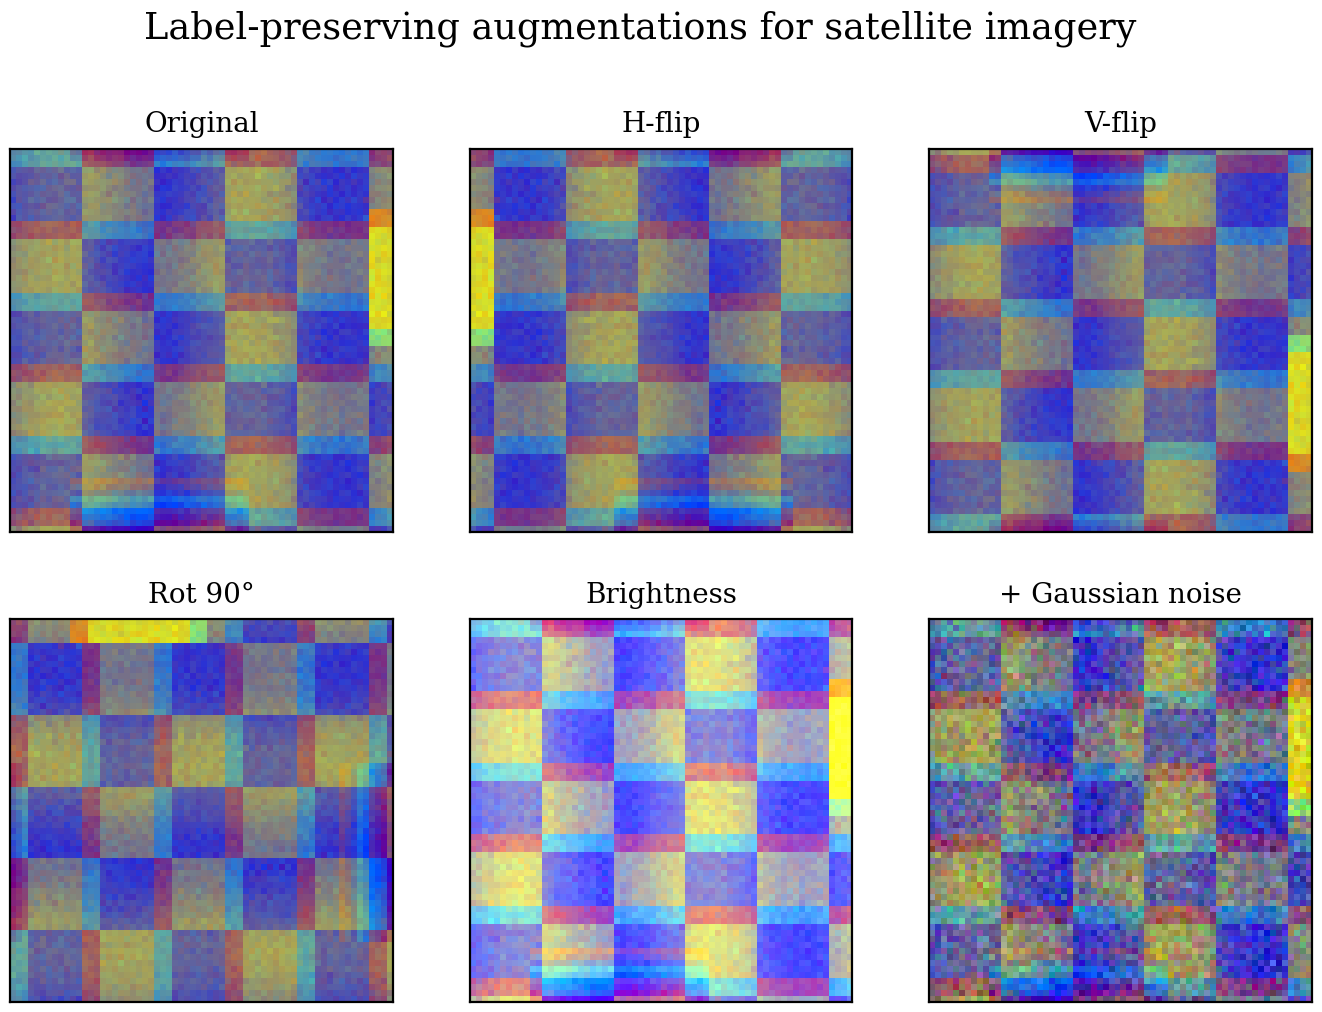
\includegraphics[width=0.86\linewidth]{figures/augmentation.png}
\caption{Label-preserving augmentations. Flips and 90° rotations are exactly
valid for nadir imagery; brightness/contrast jitter and mild Gaussian noise
simulate illumination and sensor variation.}
\label{fig:aug}
\end{figure}

\section{A pipeline with albumentations}

\texttt{albumentations} is fast, supports many bands, and --- crucially for
segmentation --- transforms image and mask jointly. A typical classification
pipeline:
\begin{lstlisting}
import albumentations as A
train_tf = A.Compose([
    A.HorizontalFlip(p=0.5),
    A.VerticalFlip(p=0.5),
    A.RandomRotate90(p=0.5),
    A.RandomBrightnessContrast(0.2, 0.2, p=0.5),
    A.GaussNoise(var_limit=(10, 50), p=0.3),
    A.Normalize(mean=MEAN, std=STD),
])
\end{lstlisting}
Validation/test pipelines contain \emph{only} normalization --- never randomise
the data you measure on.

\paragraph{What to avoid.} Augmentations that break physical meaning hurt EO
models: large hue shifts destroy the spectral signatures that distinguish
materials; heavy elastic/perspective warps fabricate impossible geometry;
aggressive blur erases the texture cues the network relies on. Prefer mild,
physically plausible photometric jitter and rely on the free geometric
invariances.

\section{Joint image--mask augmentation}

For segmentation, every geometric transform applied to the image \emph{must} be
applied identically to the label mask; photometric transforms apply to the image
only. \texttt{albumentations} handles this when you pass both:
\begin{lstlisting}
aug = A.Compose([A.HorizontalFlip(p=0.5), A.RandomRotate90(p=0.5),
                 A.RandomBrightnessContrast(p=0.5)])
out = aug(image=img, mask=mask)          # geometric ops applied to both
img_a, mask_a = out["image"], out["mask"]
\end{lstlisting}
Use nearest-neighbour interpolation for masks (labels are categorical, never
interpolate class indices) and bilinear for images.

\section{MixUp and CutMix}

These mix \emph{pairs} of examples and their labels, regularising decision
boundaries. \emph{MixUp} blends two samples linearly:
\begin{equation}
\tilde{x} = \lambda x_i + (1-\lambda) x_j, \qquad
\tilde{y} = \lambda y_i + (1-\lambda) y_j, \qquad \lambda\sim\mathrm{Beta}(\alpha,\alpha).
\end{equation}
\emph{CutMix} instead pastes a rectangular patch of one image into another and
sets the label mixing coefficient to the patch's area fraction. Both improve
calibration and robustness for classification; for segmentation, CutMix-style
region pasting is more natural than pixel blending. Use them as a complement to,
not a replacement for, geometric augmentation.

\section{Proving it works: an ablation}

Augmentation's value should be measured, not assumed. Train the same model for a
few epochs under increasing augmentation (none $\to$ geometric $\to$
geometric+photometric $\to$ +MixUp) and plot validation accuracy/mIoU. On EO
data the geometric step alone typically yields a clear gain, and the gain grows
as the labelled set shrinks --- the same low-data story as transfer learning.

\begin{keybox}
\begin{itemize}[leftmargin=1.2em,nosep]
  \item Nadir imagery $\Rightarrow$ flips + 90° rotations are exactly label-preserving (8 free views).
  \item Only normalize at validation/test time; never randomise evaluation data.
  \item Avoid hue shifts/heavy warps/blur that destroy spectral or texture cues.
  \item Segmentation: apply geometric ops to image \emph{and} mask (nearest-neighbour for masks).
  \item MixUp/CutMix mix samples and labels; complement geometric augmentation.
\end{itemize}
\end{keybox}

\begin{practbox}
Notebook: \nbpath{chapter\_08\_augmentation/08\_practical\_augmentation\_pipeline.ipynb}.
\begin{enumerate}[leftmargin=1.4em,nosep]
  \item Showcase each transform on one EuroSAT image in a grid.
  \item Build an EO-aware \texttt{albumentations} pipeline; visualise eight random
  draws of one patch.
  \item Demonstrate joint image+mask augmentation on a LoveDA sample.
  \item Implement MixUp and visualise a blended pair with its soft label.
  \item Run a 3-epoch ablation (no-aug vs aug) and plot the accuracy gain.
\end{enumerate}
\end{practbox}

\begin{exbox}
\textbf{8.1 Policy search.} Grid over augmentation strengths; find the policy
maximising validation accuracy without underfitting.\\[2pt]
\textbf{8.2 Custom EO transform.} Implement a band-wise reflectance-jitter
transform that perturbs each band independently within physical bounds.\\[2pt]
\textbf{8.3 Mask safety.} Construct a case where bilinear mask interpolation
creates invalid class indices; fix it with nearest-neighbour.\\[2pt]
\textbf{Mini-project.} Build \texttt{get\_train\_transforms(task, bands)} returning
classification and segmentation pipelines (RGB and multispectral variants) and
document each choice.
\end{exbox}


\part{Segmentation and Geospatial Pipelines}
\chapter{Semantic Segmentation and the U-Net}
\label{ch:seg}

\chapmeta{Intermediate $\to$ Advanced}{$\sim$6\,h (2.5\,h + 3.5\,h)}{LoveDA (torchgeo)}

\begin{objbox}
\begin{itemize}[leftmargin=1.2em,nosep]
  \item Reframe the task from one label per image to one label per pixel.
  \item Understand the encoder--decoder design and the role of skip connections.
  \item Implement a U-Net from scratch and trace its tensor shapes.
  \item Choose and combine segmentation losses (cross-entropy, Dice).
  \item Train and evaluate a U-Net on the LoveDA land-cover dataset.
\end{itemize}
\end{objbox}

\section{From classification to dense prediction}

Classification answers ``what is in this patch?'' with a single label.
\emph{Semantic segmentation} answers ``what is at every pixel?'', producing an
output of shape $(K,H,W)$ --- a per-pixel class distribution at full input
resolution. The challenge is that the classification encoder repeatedly
\emph{downsamples} (for receptive field and efficiency), so we must recover
spatial detail. The encoder--decoder family does this: an encoder contracts to a
compact, semantically rich representation, and a decoder expands back to full
resolution. The decoder upsamples with transposed convolutions or
interpolation+convolution; the key difficulty is that pooling has discarded the
fine localisation information the decoder needs.

\section{The U-Net architecture}

U-Net (Ronneberger et al., 2015) solves this with \emph{skip connections} that
carry high-resolution encoder feature maps directly to the matching decoder
stage, concatenating them before each decoder convolution
(Figure~\ref{fig:unet}). The encoder provides ``what''; the skips restore
``where''. This single idea is why U-Net dominates medical and EO segmentation.

\begin{figure}[h]
\centering
\begin{tikzpicture}[font=\scriptsize,>=Latex,node distance=4mm]
  \tikzstyle{enc}=[draw,fill=eoblue!12,minimum width=7mm]
  \tikzstyle{dec}=[draw,fill=eogreen!14,minimum width=7mm]
  \tikzstyle{bott}=[draw,fill=eoearth!18,minimum width=7mm]
  % encoder (heights shrink), placed left going down
  \node[enc,minimum height=22mm] (e1) {};
  \node[below=10mm of e1.south,enc,minimum height=16mm,anchor=north] (e2) {};
  \node[below=10mm of e2.south,enc,minimum height=11mm,anchor=north] (e3) {};
  \node[below=10mm of e3.south,bott,minimum height=7mm,anchor=north] (b) {};
  % decoder (heights grow), to the right
  \node[right=42mm of e3,dec,minimum height=11mm] (d3) {};
  \node[above=10mm of d3.north,dec,minimum height=16mm,anchor=south] (d2) {};
  \node[above=10mm of d2.north,dec,minimum height=22mm,anchor=south] (d1) {};
  \node[right=4mm of d1,draw,fill=eored!18,minimum height=22mm,minimum width=5mm] (out) {};
  % down arrows
  \draw[->] (e1.south) -- (e2.north) node[midway,right]{pool};
  \draw[->] (e2.south) -- (e3.north) node[midway,right]{pool};
  \draw[->] (e3.south) -- (b.north) node[midway,right]{pool};
  % up arrows
  \draw[->] (b.east) -| ($(b.east)!0.5!(d3.west)$) |- (d3.west) node[pos=0.9,above]{up};
  \draw[->] (d3.north) -- (d2.south) node[midway,right]{up};
  \draw[->] (d2.north) -- (d1.south) node[midway,right]{up};
  \draw[->] (d1.east) -- (out.west) node[midway,above]{$1\times1$};
  % skip connections
  \draw[->,eored,thick,dashed] (e1.east) -- (d1.west) node[midway,above,black]{skip (concat)};
  \draw[->,eored,thick,dashed] (e2.east) -- (d2.west);
  \draw[->,eored,thick,dashed] (e3.east) -- (d3.west);
  \node[above=1mm of e1]{encoder}; \node[above=1mm of d1]{decoder};
  \node[below=1mm of b]{bottleneck};
  \node[right=0.5mm of out]{\rotatebox{-90}{$K{\times}H{\times}W$ logits}};
\end{tikzpicture}
\caption{U-Net. The encoder (blue) halves resolution and doubles channels at
each stage; the decoder (green) mirrors it, upsampling and halving channels.
Dashed red skip connections concatenate same-resolution encoder features into
the decoder, restoring spatial detail lost to pooling. A final $1\times1$
convolution maps to $K$ class logits per pixel.}
\label{fig:unet}
\end{figure}

A minimal from-scratch U-Net uses a reusable double-convolution block:
\begin{lstlisting}
import torch, torch.nn as nn
class DoubleConv(nn.Module):
    def __init__(self, cin, cout):
        super().__init__()
        self.net = nn.Sequential(
            nn.Conv2d(cin, cout, 3, padding=1, bias=False),
            nn.BatchNorm2d(cout), nn.ReLU(inplace=True),
            nn.Conv2d(cout, cout, 3, padding=1, bias=False),
            nn.BatchNorm2d(cout), nn.ReLU(inplace=True))
    def forward(self, x): return self.net(x)

class Up(nn.Module):
    def __init__(self, cin, cout):
        super().__init__()
        self.up = nn.ConvTranspose2d(cin, cin // 2, 2, stride=2)
        self.conv = DoubleConv(cin, cout)            # cin = up + skip channels
    def forward(self, x, skip):
        x = self.up(x)
        x = torch.cat([skip, x], dim=1)              # concatenate skip
        return self.conv(x)
\end{lstlisting}
Tracing shapes for a $256\times256$ input with base width 64: the encoder
produces feature maps at $256,128,64,32$ resolutions with $64,128,256,512$
channels; the decoder reverses this, each \texttt{Up} consuming the matching
skip; the head outputs $(K,256,256)$.

\section{Loss functions for segmentation}

Per-pixel cross-entropy (Eq.~\ref{eq:ce}, summed over pixels) is the baseline,
but land-cover classes are imbalanced (water and bare soil are rare), and CE is
dominated by frequent classes. The \emph{Dice loss} directly optimises overlap
and is robust to imbalance. For predicted soft probabilities $p$ and one-hot
target $g$ over $N$ pixels and class $k$:
\begin{equation}
\mathcal{L}_{\mathrm{Dice}} = 1 - \frac{1}{K}\sum_{k=1}^{K}
\frac{2\sum_i p_{ik}\,g_{ik} + \varepsilon}{\sum_i p_{ik} + \sum_i g_{ik} + \varepsilon}.
\label{eq:dice}
\end{equation}
In practice a \emph{combined} loss works best, pairing CE's well-behaved
gradients with Dice's overlap objective:
\begin{equation}
\mathcal{L} = \mathcal{L}_{\mathrm{CE}} + \lambda\,\mathcal{L}_{\mathrm{Dice}},
\qquad \lambda \approx 1.
\end{equation}
For severe imbalance, class-weighted CE or focal loss (down-weighting easy
pixels) are alternatives. We measure success with IoU/mIoU, defined in
Chapter~\ref{ch:eval}.

\section{Training on LoveDA}

LoveDA (Wang et al., 2021) provides 5{,}987 high-resolution
($1024\times1024$) scenes over urban and rural domains with seven land-cover
classes, auto-downloaded via \texttt{torchgeo}. The recipe combines everything
so far: tile to $512\times512$ (Chapter~\ref{ch:preproc}), augment image+mask
jointly (Chapter~\ref{ch:aug}), use a U-Net (optionally with a pretrained
encoder, Chapter~\ref{ch:transfer}), optimise the combined loss, and checkpoint
on validation mIoU. The ablation that most convinces students: train the U-Net
\emph{with} and \emph{without} skip connections --- the no-skip variant produces
blurry, mislocalised masks and markedly lower mIoU, making the role of the skips
concrete.

\begin{keybox}
\begin{itemize}[leftmargin=1.2em,nosep]
  \item Segmentation outputs $(K,H,W)$: a class distribution per pixel.
  \item Encoder--decoder recovers resolution; skip connections restore localisation (``what'' + ``where'').
  \item Decoder upsamples via transposed conv (or interpolate+conv) and concatenates skips.
  \item Combine cross-entropy with Dice (Eq.~\ref{eq:dice}) for imbalanced land cover.
  \item Pretrained encoders and joint image+mask augmentation carry straight over from earlier chapters.
\end{itemize}
\end{keybox}

\begin{practbox}
Notebook: \nbpath{chapter\_09\_semantic\_segmentation/09\_practical\_unet\_segmentation.ipynb}.
\begin{enumerate}[leftmargin=1.4em,nosep]
  \item Implement \texttt{DoubleConv}, \texttt{Down}, \texttt{Up}, \texttt{OutConv}
  and assemble a U-Net; print feature-map shapes at every stage.
  \item Implement Dice loss and the combined CE+Dice loss.
  \item Load LoveDA via \texttt{torchgeo}; build a segmentation \texttt{DataLoader}
  with joint augmentation; visualise image/mask pairs.
  \item Train for several epochs; plot loss and validation mIoU curves.
  \item Load the best model and display RGB\,$|$\,GT\,$|$\,prediction triplets.
\end{enumerate}
\end{practbox}

\begin{exbox}
\textbf{9.1 No-skip ablation.} Remove the skip connections; quantify the mIoU
drop and show the blurrier masks.\\[2pt]
\textbf{9.2 Loss comparison.} Train with CE only, Dice only, and CE+Dice; compare
per-class IoU, especially on rare classes.\\[2pt]
\textbf{9.3 Depth/width.} Vary U-Net depth and base width; relate capacity to
mIoU and memory.\\[2pt]
\textbf{Mini-project.} Add an ImageNet-pretrained ResNet encoder to your U-Net
(manual or via SMP, Chapter~\ref{ch:advseg}) and measure the mIoU gain over the
from-scratch version.
\end{exbox}

\chapter{Advanced Segmentation Architectures}
\label{ch:advseg}

\chapmeta{Advanced}{$\sim$5\,h (2\,h + 3\,h)}{LoveDA}

\begin{objbox}
\begin{itemize}[leftmargin=1.2em,nosep]
  \item Use \texttt{segmentation-models-pytorch} (SMP) to build decoders on pretrained encoders.
  \item Understand atrous (dilated) convolution and DeepLabV3+'s ASPP module.
  \item Understand multi-scale context: FPN and PSPNet pyramid pooling.
  \item Benchmark architectures fairly on a common dataset and budget.
  \item Choose an architecture/encoder for a given EO constraint.
\end{itemize}
\end{objbox}

The hand-built U-Net of Chapter~\ref{ch:seg} taught the mechanics. In practice
we assemble decoders on top of pretrained encoders with a library, and choose
among architectures designed to capture \emph{multi-scale context} --- essential
in EO, where land-cover objects range from single trees to whole agricultural
regions.

\section{segmentation-models-pytorch}

SMP exposes every architecture through one uniform constructor, pairing a
decoder with any of dozens of pretrained encoders (\texttt{timm}-backed):
\begin{lstlisting}
import segmentation_models_pytorch as smp
model = smp.Unet(encoder_name="resnet50", encoder_weights="imagenet",
                 in_channels=3, classes=7)
# swap decoder by changing the class: smp.DeepLabV3Plus / smp.FPN / smp.PSPNet
\end{lstlisting}
For multispectral input set \texttt{in\_channels=13}; SMP adapts the first
convolution automatically (cf.\ Chapter~\ref{ch:transfer}). This one-line
flexibility is what makes principled architecture comparison feasible.

\section{Atrous convolution and DeepLabV3+}

A standard convolution must pool to enlarge its receptive field, sacrificing
resolution. \emph{Atrous} (dilated) convolution inserts gaps of rate $r$ between
kernel taps, enlarging the receptive field \emph{without} downsampling or extra
parameters. A dilated $k\times k$ kernel has an effective size
\begin{equation}
k_\mathrm{eff} = k + (k-1)(r-1),
\end{equation}
so a $3\times3$ kernel at rate $r{=}6$ covers $13\times13$. DeepLabV3+ uses
\emph{Atrous Spatial Pyramid Pooling} (ASPP): several parallel atrous
convolutions at different rates (e.g.\ $6,12,18$) plus image-level global
pooling, concatenated to fuse context at multiple scales, followed by a light
decoder that recovers boundaries. It excels when objects span very different
sizes --- the norm in land cover.

\section{FPN and PSPNet}

\emph{Feature Pyramid Networks} (FPN) build a top-down pathway with lateral
connections, producing semantically strong features at every resolution and
fusing predictions across the pyramid --- naturally multi-scale and efficient.
\emph{PSPNet} introduces the \emph{pyramid pooling module}, pooling the deepest
feature map at several grid scales ($1\times1, 2\times2, 3\times3, 6\times6$),
processing each, and concatenating, injecting global scene context that helps
disambiguate locally-similar classes (e.g.\ shadowed roof vs water). All three
--- DeepLabV3+, FPN, PSPNet --- attack the same problem (context at multiple
scales) by different means.

\section{A fair benchmark}

Comparisons are only meaningful under a fixed protocol: same encoder, same data
splits, same augmentation, same epochs and optimiser, varying only the decoder.
Report mIoU, parameters, and inference latency.

\begin{center}\small
\renewcommand{\arraystretch}{1.2}
\begin{tabular}{@{}lllll@{}}
\toprule
Decoder & Context mechanism & Params & Strength & Typical use\\
\midrule
U-Net & skip connections & low--med & sharp boundaries & default, small data\\
FPN & feature pyramid & low & multi-scale, fast & efficient inference\\
PSPNet & pyramid pooling & med & global context & scene-level classes\\
DeepLabV3+ & ASPP (atrous) & med--high & multi-scale + edges & best all-round\\
\bottomrule
\end{tabular}
\end{center}

\noindent On LoveDA with a ResNet50 encoder the four are usually within a few
mIoU points; DeepLabV3+ tends to lead on boundary-heavy urban scenes, U-Net
remains a strong, low-memory default, and FPN is attractive when latency
matters. The lesson is to \emph{measure on your data and budget} rather than
trust leaderboard ranks from another domain.

\begin{keybox}
\begin{itemize}[leftmargin=1.2em,nosep]
  \item SMP $=$ decoder $\times$ pretrained encoder via one constructor; trivial multispectral support.
  \item Atrous convolution grows the receptive field without losing resolution; $k_\mathrm{eff}=k+(k-1)(r-1)$.
  \item DeepLabV3+ (ASPP), FPN and PSPNet all capture multi-scale context differently.
  \item Benchmark fairly: fix everything but the decoder; report mIoU, params, latency.
  \item No universal winner --- choose for your data, objects' scale, and compute budget.
\end{itemize}
\end{keybox}

\begin{practbox}
Notebook: \nbpath{chapter\_10\_advanced\_segmentation/10\_practical\_advanced\_segmentation.ipynb}.
\begin{enumerate}[leftmargin=1.4em,nosep]
  \item Build U-Net, DeepLabV3+, FPN and PSPNet with SMP on a shared ResNet50
  encoder; print parameter counts.
  \item Visualise how atrous rate enlarges the receptive field.
  \item Run a fixed-protocol benchmark of the four decoders for a few epochs.
  \item Plot mIoU vs params vs latency; pick a winner.
  \item Train the winner longer and display prediction triplets.
\end{enumerate}
\end{practbox}

\begin{exbox}
\textbf{10.1 Encoder swap.} Hold the decoder fixed and compare ResNet34/50 and
EfficientNet-B0/B4 encoders by mIoU and speed.\\[2pt]
\textbf{10.2 ASPP rates.} Vary DeepLab's atrous rates; relate them to the object
scales in LoveDA.\\[2pt]
\textbf{10.3 Multispectral.} Rebuild the best model with \texttt{in\_channels=13}
on a multispectral dataset; measure the gain over RGB.\\[2pt]
\textbf{Mini-project.} Produce a one-page ``architecture selection'' report
recommending a decoder+encoder for (a) a latency-constrained edge device and (b)
a maximum-accuracy server, justified by your benchmark.
\end{exbox}

\chapter{The Full EO Pipeline: Tiling, Inference, GeoTIFF}
\label{ch:pipeline}

\chapmeta{Advanced}{$\sim$6\,h (2\,h + 4\,h)}{Sentinel-2 scenes (synthetic + real)}

\begin{objbox}
\begin{itemize}[leftmargin=1.2em,nosep]
  \item Assemble a complete pipeline: raw scene $\to$ tiles $\to$ inference $\to$ map.
  \item Implement memory-safe sliding-window inference over a full Sentinel-2 tile.
  \item Blend overlapping predictions with Gaussian weighting to remove seams.
  \item Export a georeferenced GeoTIFF with correct CRS and transform.
  \item Compute per-class area statistics from a prediction map.
\end{itemize}
\end{objbox}

This chapter closes the loop: a trained segmentation model becomes a deployable
system that turns a $\sim$$10980\times10980$ Sentinel-2 scene into a
georeferenced land-cover map. No single GPU can hold such a scene, so inference
must be tiled, and the tiles' predictions stitched back into one seamless raster.

\section{Pipeline overview}

The end-to-end flow chains the components built in earlier chapters
(Figure~\ref{fig:pipe}): load and preprocess the scene
(Chapter~\ref{ch:preproc}), tile it with overlap, run the model on each tile
(Chapters~\ref{ch:seg}--\ref{ch:advseg}), blend predictions, reconstruct the
full map, and write a GeoTIFF.

\begin{figure}[h]
\centering
\begin{tikzpicture}[font=\scriptsize,>=Latex,node distance=5mm]
  \tikzstyle{b}=[draw,rounded corners,minimum height=8mm,minimum width=20mm,align=center]
  \node[b,fill=eoblue!10] (a){Raw scene\\(GeoTIFF)};
  \node[b,fill=eoblue!10,right=of a] (p){Preprocess\\norm + indices};
  \node[b,fill=eoearth!12,right=of p] (t){Tile\\(overlap)};
  \node[b,fill=eogreen!12,right=of t] (m){Model\\per tile};
  \node[b,fill=eogreen!12,below=7mm of m] (bl){Gaussian\\blend};
  \node[b,fill=eoearth!12,left=of bl] (rc){Reconstruct\\full map};
  \node[b,fill=eored!12,left=of rc] (g){Export\\GeoTIFF};
  \draw[->](a)--(p);\draw[->](p)--(t);\draw[->](t)--(m);\draw[->](m)--(bl);
  \draw[->](bl)--(rc);\draw[->](rc)--(g);
\end{tikzpicture}
\caption{The full inference pipeline. Every stage corresponds to a tool built in
an earlier chapter; only the orchestration is new.}
\label{fig:pipe}
\end{figure}

\section{Sliding-window inference}

We slide a $T\times T$ window with stride $s<T$ (overlap $T-s$) across the
scene. For each window we run the model to obtain class \emph{probabilities}
(not hard labels --- we need to average), and accumulate them into a full-scene
buffer $P\in\R^{K\times H\times W}$ together with a weight buffer $A$. The final
per-pixel prediction is $\arg\max_k P[k]/A$.
\begin{lstlisting}
import numpy as np, torch
def sliding_window(model, scene, T=512, s=384, K=7, device="cuda"):
    C, H, W = scene.shape
    P = np.zeros((K, H, W), np.float32); A = np.zeros((H, W), np.float32)
    wmap = gaussian_weight(T)                      # (T, T), peaks at centre
    model.eval()
    with torch.no_grad():
        for y in range(0, H - T + 1, s):
            for x in range(0, W - T + 1, s):
                tile = torch.from_numpy(scene[:, y:y+T, x:x+T])[None].to(device)
                prob = model(tile).softmax(1)[0].cpu().numpy()   # (K, T, T)
                P[:, y:y+T, x:x+T] += prob * wmap
                A[y:y+T, x:x+T]    += wmap
    return (P / np.maximum(A, 1e-6)).argmax(0)     # (H, W) labels
\end{lstlisting}
Edge handling (padding the last partial tile) and batching multiple tiles
together for throughput are the practical refinements.

\section{Why Gaussian blending}

If overlapping tiles are averaged with equal weight, predictions near a tile's
border --- where the receptive field is truncated and context is missing --- are
unreliable and produce visible grid \emph{seams}. Weighting each tile by a 2D
Gaussian $w(u,v)\propto\exp\!\big(-\tfrac{(u-c)^2+(v-c)^2}{2\sigma^2}\big)$
centred on the tile (so centre pixels dominate, borders fade) makes the
contributions of adjacent tiles transition smoothly, eliminating seams. The
ablation ``equal weight vs Gaussian'' makes the artefact and its cure obvious.

\section{Georeferenced export}

A prediction is useless to a GIS analyst unless it carries its geolocation. We
write the label raster with the \emph{same} CRS and affine transform as the
input scene, so it overlays exactly in QGIS:
\begin{lstlisting}
import rasterio
with rasterio.open(src_path) as src:
    profile = src.profile
profile.update(count=1, dtype="uint8", nodata=0)
with rasterio.open("landcover.tif", "w", **profile) as dst:
    dst.write(pred.astype("uint8"), 1)
    dst.write_colormap(1, {i: hex_to_rgb(c) for i, c in enumerate(PALETTE)})
\end{lstlisting}
Embedding a colour map renders the classes correctly without manual styling.

\section{Area statistics}

Because each pixel covers a known ground area ($10\times10\,\mathrm{m}=100\,
\mathrm{m}^2$ for Sentinel-2 10\,m bands), counting pixels per class converts
directly to hectares:
\begin{equation}
\text{area}_k\,[\mathrm{ha}] = \frac{n_k \cdot A_\mathrm{px}}{10^4},
\qquad A_\mathrm{px}=|a\cdot e|\ \mathrm{m}^2,
\end{equation}
turning a colourful map into the quantitative output stakeholders actually want
(``X hectares of forest, Y of built-up''). Figure~\ref{fig:lc} shows a
representative scene and its predicted land-cover map.

\begin{figure}[h]
\centering
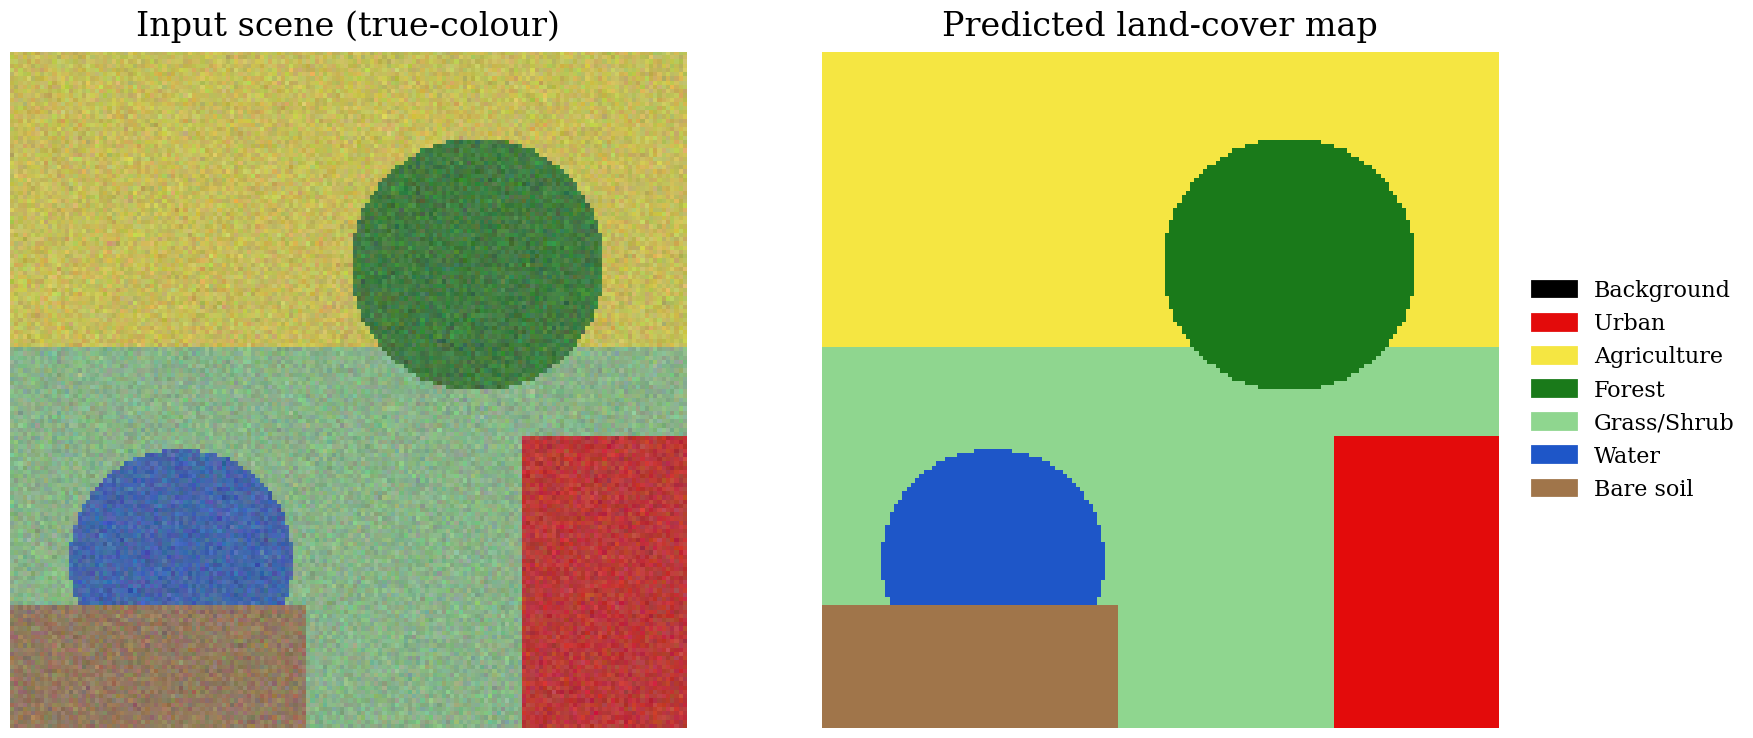
\includegraphics[width=0.95\linewidth]{figures/landcover.png}
\caption{Input scene (left) and reconstructed land-cover prediction (right) with
a class legend --- the deliverable of the full pipeline and of the capstone.}
\label{fig:lc}
\end{figure}

\begin{keybox}
\begin{itemize}[leftmargin=1.2em,nosep]
  \item Full-scene inference is tiled; accumulate \emph{probabilities}, then argmax.
  \item Overlap + Gaussian blending removes tile seams from truncated-context borders.
  \item Export with the source CRS/transform (and a colour map) for GIS-ready GeoTIFFs.
  \item Pixel area $\to$ hectares gives quantitative, decision-ready statistics.
  \item The pipeline is pure orchestration of tools from Chapters~\ref{ch:preproc}--\ref{ch:advseg}.
\end{itemize}
\end{keybox}

\begin{practbox}
Notebook: \nbpath{chapter\_11\_full\_eo\_pipeline/11\_practical\_end\_to\_end\_pipeline.ipynb}.
\begin{enumerate}[leftmargin=1.4em,nosep]
  \item Create (or load) a large multi-band scene with spatial structure.
  \item Implement \texttt{gaussian\_weight} and the sliding-window inference loop.
  \item Run inference with a trained (or demo) model; reconstruct the full map.
  \item Compare reconstructions \emph{with} and \emph{without} Gaussian blending.
  \item Export a georeferenced GeoTIFF with a colour map; compute per-class hectares.
\end{enumerate}
\end{practbox}

\begin{exbox}
\textbf{11.1 Overlap effect.} Sweep stride/overlap; quantify seam artefacts and
runtime trade-offs.\\[2pt]
\textbf{11.2 Batched tiles.} Batch multiple tiles per forward pass; measure the
throughput gain.\\[2pt]
\textbf{11.3 QGIS check.} Open your GeoTIFF in QGIS over an OSM basemap; verify
alignment and discuss any offset.\\[2pt]
\textbf{Mini-project.} Wrap the pipeline into \texttt{predict\_scene(model,
path) -> geotiff} with a CLI, then run it on a real downloaded Sentinel-2 tile.
\end{exbox}

\chapter{Evaluation and Interpretability}
\label{ch:eval}

\chapmeta{Advanced}{$\sim$4\,h (2\,h + 2\,h)}{LoveDA; trained checkpoints}

\begin{objbox}
\begin{itemize}[leftmargin=1.2em,nosep]
  \item Define and compute IoU, mIoU, Dice, pixel accuracy and per-class F1.
  \item Build and correctly normalise a confusion matrix for segmentation.
  \item Apply GradCAM to see where a CNN ``looks''.
  \item Use prediction-entropy maps to flag uncertain regions.
  \item Conduct a structured failure analysis and propose targeted fixes.
\end{itemize}
\end{objbox}

A land-cover map is only as trustworthy as its evaluation. This chapter
formalises the metrics used throughout the course and adds interpretability
tools that turn ``the mIoU is 0.58'' into actionable understanding of \emph{where}
and \emph{why} the model fails.

\section{Segmentation metrics}

Let TP, FP, FN be the per-class pixel counts. The \emph{Intersection over Union}
(Jaccard index) for class $k$ and its mean over classes are
\begin{equation}
\mathrm{IoU}_k = \frac{\mathrm{TP}_k}{\mathrm{TP}_k+\mathrm{FP}_k+\mathrm{FN}_k},
\qquad
\mathrm{mIoU} = \frac{1}{K}\sum_{k=1}^{K}\mathrm{IoU}_k.
\label{eq:iou}
\end{equation}
mIoU is the standard segmentation headline because, unlike pixel accuracy, it
weights every class equally and is not inflated by a dominant background. The
\emph{Dice} (F1) coefficient is closely related,
\begin{equation}
\mathrm{Dice}_k = \frac{2\,\mathrm{TP}_k}{2\,\mathrm{TP}_k+\mathrm{FP}_k+\mathrm{FN}_k}
= \frac{2\,\mathrm{IoU}_k}{1+\mathrm{IoU}_k},
\end{equation}
always at least as large as IoU and more forgiving of small errors
(Figure~\ref{fig:iou}). \emph{Pixel accuracy} (fraction of correctly labelled
pixels) is reported for completeness but is misleading under class imbalance.

\begin{figure}[h]
\centering
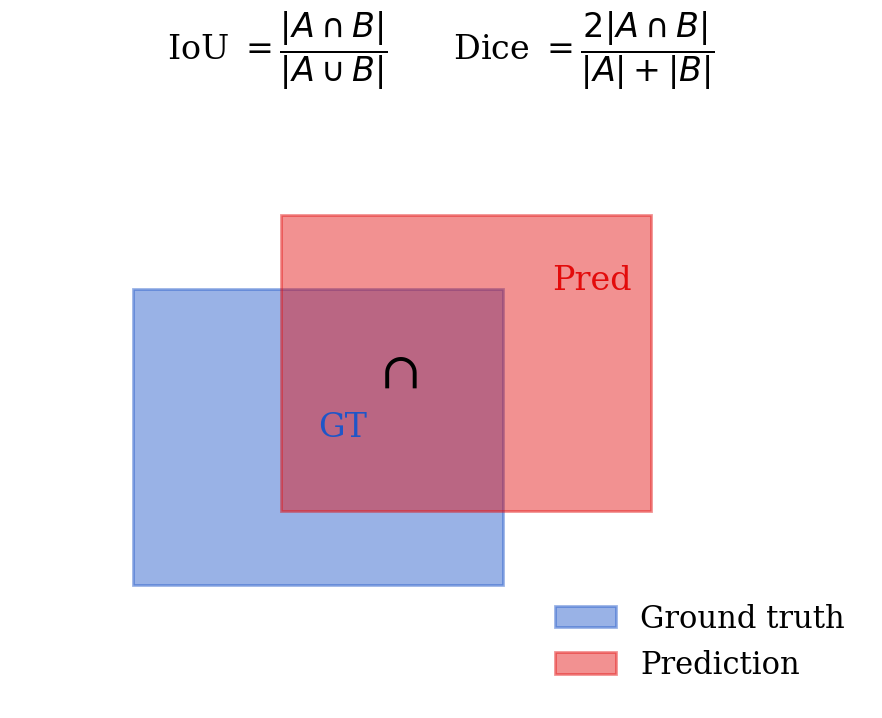
\includegraphics[width=0.62\linewidth]{figures/iou.png}
\caption{IoU and Dice for a predicted region (red) versus ground truth (blue).
IoU divides intersection by union; Dice doubles the intersection over the sum of
areas. Both reward overlap and penalise both false positives and false
negatives.}
\label{fig:iou}
\end{figure}

\section{The confusion matrix}

The $K\times K$ confusion matrix $C$, with $C_{ij}$ the number of pixels of true
class $i$ predicted as $j$, is the richest single diagnostic. \emph{Row-normalise}
it ($C_{ij}/\sum_j C_{ij}$) to read per-class recall and to see which classes are
confused for which (Figure~\ref{fig:cm}). In land cover the off-diagonal mass
concentrates among semantically adjacent classes --- grassland vs agriculture,
urban vs bare soil --- which points directly at where extra bands, indices or
augmentation would help.

\begin{figure}[h]
\centering
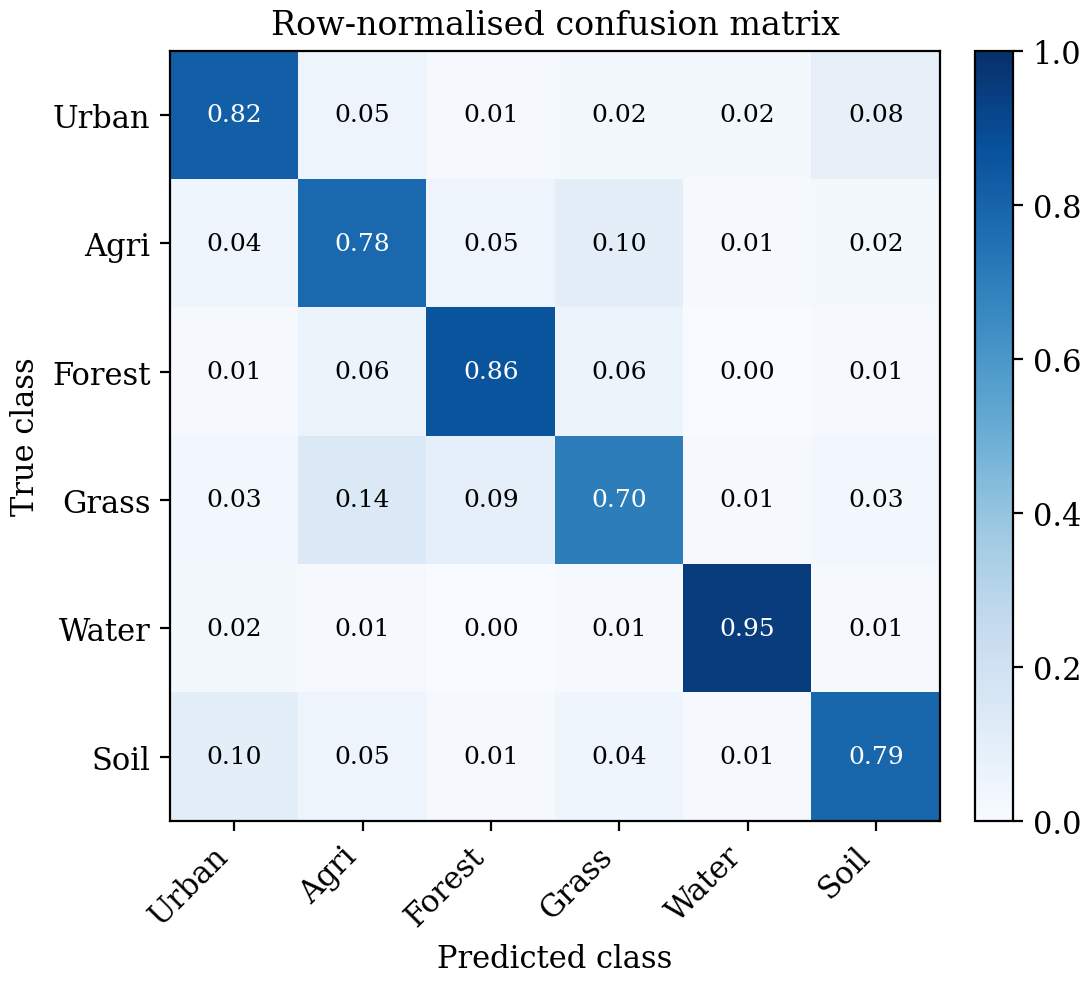
\includegraphics[width=0.52\linewidth]{figures/confusion.png}
\caption{Row-normalised confusion matrix. The diagonal is per-class recall;
bright off-diagonal cells (e.g.\ grassland $\to$ agriculture) reveal systematic,
explainable confusions to target.}
\label{fig:cm}
\end{figure}

\section{GradCAM: what the model sees}

GradCAM produces a coarse heat-map of the image regions most responsible for a
prediction. For target class $c$ and the activations $A^{k}$ of a chosen
convolutional layer, the neuron-importance weights are the
gradient-global-average
\begin{equation}
\alpha^{c}_{k} = \frac{1}{Z}\sum_{i,j}\frac{\partial y^{c}}{\partial A^{k}_{ij}},
\qquad
L^{c}_{\mathrm{GradCAM}} = \mathrm{ReLU}\!\Big(\sum_{k}\alpha^{c}_{k} A^{k}\Big),
\end{equation}
upsampled to the input size. For EO it answers questions like ``did the network
classify this patch as \textsf{Industrial} because of the buildings or because of
an adjacent road?'', exposing spurious correlations (a model keying on image
borders or compression artefacts is a real failure mode).

\section{Uncertainty via entropy}

The per-pixel predictive entropy of the softmax distribution,
\begin{equation}
\mathcal{H}(\mathbf{p}) = -\sum_{k=1}^{K} p_k \log p_k,
\end{equation}
is a cheap uncertainty proxy: high entropy marks pixels where the model hedges
--- typically class boundaries and genuinely ambiguous land cover. An entropy
\emph{map} overlaid on the prediction shows reviewers exactly where to look and
is the basis of active-learning sample selection.

\section{Failure analysis}

Good practice closes the loop: rank validation tiles by error, inspect the worst,
categorise the mistakes (boundary leakage, whole-class confusion, rare-class
misses, tiling seams), attribute each to a cause, and propose a targeted fix
(class weighting for rare classes, more overlap for seams, extra indices for
spectral confusion). A short, honest discussion of failure cases is what
separates a portfolio project from a toy --- and is explicitly rewarded in the
capstone rubric.

\begin{keybox}
\begin{itemize}[leftmargin=1.2em,nosep]
  \item mIoU (Eq.~\ref{eq:iou}) is the class-balanced headline; pixel accuracy misleads under imbalance.
  \item Dice $\ge$ IoU; both penalise FP and FN.
  \item Row-normalised confusion matrices reveal \emph{which} classes are confused.
  \item GradCAM localises evidence; entropy maps localise uncertainty.
  \item Structured failure analysis turns metrics into targeted improvements.
\end{itemize}
\end{keybox}

\begin{practbox}
Notebook: \nbpath{chapter\_12\_evaluation\_interpretability/12\_practical\_evaluation\_interpretability.ipynb}.
\begin{enumerate}[leftmargin=1.4em,nosep]
  \item Implement per-class IoU, mIoU, Dice, pixel accuracy and F1 from a confusion matrix.
  \item Plot a publication-quality row-normalised confusion matrix.
  \item Apply GradCAM to a trained model for selected classes; interpret the heat-maps.
  \item Compute and visualise a prediction-entropy map.
  \item Rank tiles by error and write a short failure-mode report.
\end{enumerate}
\end{practbox}

\begin{exbox}
\textbf{12.1 IoU vs Dice.} Construct prediction/GT pairs where IoU and Dice
disagree most; explain the geometry.\\[2pt]
\textbf{12.2 Boundary metric.} Implement a boundary-IoU that scores only pixels
near class edges; compare with standard IoU.\\[2pt]
\textbf{12.3 Calibration.} Plot a reliability diagram of predicted confidence vs
accuracy; is the model over- or under-confident?\\[2pt]
\textbf{Mini-project.} Build an \texttt{evaluation\_report(model, loader)} that
emits a metrics table, confusion matrix, GradCAM panel, entropy map and a ranked
failure gallery as a single figure/markdown bundle.
\end{exbox}


\part{Capstone and Reference}
\chapter{Capstone: End-to-End Land-Cover Mapping}
\label{ch:capstone}

\chapmeta{Advanced}{$\sim$10\,h ($\sim$4 weeks part-time)}{LoveDA and/or Sentinel-2 + OSM labels}

\begin{objbox}
\begin{itemize}[leftmargin=1.2em,nosep]
  \item Integrate the entire course into one production-grade system, independently.
  \item Take a raw Sentinel-2 Level-2A scene to a georeferenced land-cover GeoTIFF.
  \item Justify every design choice (encoder, decoder, loss, augmentation).
  \item Evaluate rigorously and analyse failures.
  \item Package a portfolio-ready deliverable.
\end{itemize}
\end{objbox}

This is not a tutorial: there is no step-by-step guide. You apply everything from
Chapters~\ref{ch:intro}--\ref{ch:eval} to solve a real mapping problem on your
own. Notebook: \nbpath{notebooks/capstone/capstone\_land\_cover\_mapping.ipynb}.

\section{Problem statement}

Given a Sentinel-2 Level-2A tile (bottom-of-atmosphere reflectance, 12 usable
bands, $\sim$$110\times110$\,km), produce a pixel-level land-cover map over seven
classes.

\begin{center}\small
\renewcommand{\arraystretch}{1.15}
\begin{tabular}{@{}cll@{}}
\toprule
ID & Class & Colour\\
\midrule
0 & Background / no-data & \texttt{\#000000}\\
1 & Urban / built-up & \texttt{\#E30B0B}\\
2 & Agriculture & \texttt{\#F5E642}\\
3 & Forest & \texttt{\#1A7A1A}\\
4 & Shrubland / grassland & \texttt{\#8FD68F}\\
5 & Water & \texttt{\#1E56C8}\\
6 & Bare soil / rock & \texttt{\#A0754A}\\
\bottomrule
\end{tabular}
\end{center}

\section{Mandatory components}

\begin{description}[leftmargin=1.6em,style=nextline]
  \item[Data pipeline] load with \texttt{rasterio}/\texttt{rioxarray}; stack
  B02/B03/B04/B08 (10\,m) with B05--B07/B8A/B11/B12 (20\,m, upsampled); compute
  $\geq$2 indices (NDVI, NDWI, $\dots$); normalize with training statistics;
  generate $512\times512$ tiles with configurable overlap.
  \item[Model]   an SMP model with a pretrained encoder; justify the encoder
  (ResNet50, EfficientNet-B4 or MobileNetV3) and the decoder (U-Net, FPN or
  DeepLabV3+);
  handle class imbalance with weighted Dice or focal loss.
  \item[Training] LoveDA or Sentinel-2 + OSM-derived labels; early stopping;
  $\geq$4 augmentation types; log loss and IoU per epoch; checkpoint on best
  validation mIoU.
  \item[Evaluation] per-class IoU, mIoU, F1, overall accuracy; confusion matrix;
  $\geq$5 qualitative examples with GT overlays; GradCAM for $\geq$1 class.
  \item[Inference] sliding-window over the full tile with Gaussian blending;
  reconstruct; export a georeferenced GeoTIFF with correct CRS/transform.
  \item[Visualisation] colour-coded map with legend; true-colour vs prediction
  side-by-side; per-class area in hectares.
\end{description}

\section{Deliverables and rubric}

\begin{center}\small
\renewcommand{\arraystretch}{1.15}
\begin{tabular}{@{}lll@{}}
\toprule
Deliverable & Format & Weight\\
\midrule
End-to-end executed notebook & \texttt{.ipynb} & 40\%\\
Trained model checkpoint & \texttt{.pth} & 10\%\\
Prediction GeoTIFF (with CRS) & \texttt{.tif} & 15\%\\
Evaluation report (metrics + confusion matrix) & MD/PDF & 20\%\\
Technical writeup (max 2 pages) & PDF/MD & 15\%\\
\bottomrule
\end{tabular}
\end{center}

The 100-point rubric is split evenly across five areas --- Data pipeline, Model
architecture, Training, Evaluation, Inference+GeoTIFF (20 points each). Full
marks require not just working code but \emph{justified} choices: a silently used
default encoder scores zero on that criterion even if accurate. A validation
mIoU $\geq 40\%$ earns the evaluation points; $30$--$40\%$ partial.
Grades: Distinction $85$--$100$, Merit $70$--$84$, Pass $55$--$69$.

\begin{center}\small
\renewcommand{\arraystretch}{1.15}
\begin{tabular}{@{}ll@{}}
\toprule
Week & Focus\\
\midrule
1 & Data pipeline: loading, normalization, tiling\\
2 & Model setup, first training run, baseline metrics\\
3 & Ablations (loss functions, encoders, augmentation)\\
4 & Inference pipeline, GeoTIFF export, evaluation report\\
\bottomrule
\end{tabular}
\end{center}

\section{Extension ideas}

For a Distinction-level project, push beyond the brief:
multi-temporal fusion (stack two seasons to improve agricultural classes);
domain generalisation (train on one region, test on another, analyse the shift);
Sentinel-1 SAR fusion (add backscatter channels, measure gains on water/urban);
uncertainty via Monte-Carlo dropout; CRF post-processing for sharper boundaries;
or a Streamlit/FastAPI demo that ingests a GeoTIFF and returns a prediction map.

\section{Portfolio checklist}

\begin{itemize}[leftmargin=1.4em,nosep]
  \item Notebook runs end-to-end from a clean kernel restart.
  \item Every cell has explanatory markdown; every figure has titles, labels, legends.
  \item GeoTIFF opens and aligns correctly in QGIS.
  \item A \texttt{README} explains how to reproduce; checkpoint $<500$\,MB (Git LFS if needed).
  \item The report discusses failure cases honestly.
\end{itemize}

\begin{notebox}[The point of the capstone]
The capstone is the artefact you show an employer. A clear writeup, a
banner figure (true-colour vs prediction), an honest limitations section and a
one-line headline (``ResNet50 + DeepLabV3+, mIoU 58\% on LoveDA'') demonstrate
end-to-end competence more convincingly than any single notebook from the course.
\end{notebox}


\appendix
\chapter{Practical Infrastructure}
\label{app:infra}

This appendix collects the software, environment and hardware details needed to
run every notebook in the course.

\section{Software stack}

\begin{center}\small
\renewcommand{\arraystretch}{1.15}
\begin{tabular}{@{}lll@{}}
\toprule
Layer & Library & Version\\
\midrule
Language & Python & 3.12\\
Deep learning & PyTorch & $\geq$2.2\\
Computer vision & torchvision & $\geq$0.17\\
Segmentation & segmentation-models-pytorch & $\geq$0.3.3\\
Metrics & torchmetrics & $\geq$1.3\\
EO datasets & torchgeo & $\geq$0.6\\
Raster I/O & rasterio & $\geq$1.3\\
Raster + xarray & rioxarray & $\geq$0.15\\
Multi-dim arrays & xarray & $\geq$2024.1\\
Vector + CRS & geopandas & $\geq$0.14\\
Augmentation & albumentations & $\geq$1.4\\
Visualisation & matplotlib / seaborn & latest\\
Interpretability & pytorch-grad-cam & $\geq$1.5\\
Notebooks & jupyterlab & $\geq$4.1\\
\bottomrule
\end{tabular}
\end{center}

\section{Environment setup}

\paragraph{uv (recommended).}
\begin{lstlisting}
curl -LsSf https://astral.sh/uv/install.sh | sh
git clone <repo-url> CNN_projects && cd CNN_projects
uv sync                 # installs from pyproject.toml into .venv
uv run jupyter lab
\end{lstlisting}

\paragraph{conda or pip.}
\begin{lstlisting}
conda env create -f environment.yml && conda activate eo-cnn && pip install -e .
# or
python3.12 -m venv .venv && source .venv/bin/activate
pip install -r requirements.txt && pip install -e .
\end{lstlisting}

\paragraph{Google Colab.} Every notebook begins with a setup cell that installs
dependencies, mounts Drive, and detects the device:
\begin{lstlisting}
IN_COLAB = 'google.colab' in str(get_ipython())
if IN_COLAB:
    !pip install -q torch torchvision torchgeo segmentation-models-pytorch \
                    torchmetrics albumentations rasterio rioxarray geopandas grad-cam tqdm
    from google.colab import drive; drive.mount('/content/drive')
    DATA_ROOT = '/content/drive/MyDrive/eo_cnn_data'
else:
    DATA_ROOT = '../data'
DEVICE = 'cuda' if torch.cuda.is_available() else 'cpu'
FAST_MODE = not torch.cuda.is_available()   # reduces epochs/data on CPU
\end{lstlisting}

\section{Repository structure}

\begin{lstlisting}
CNN_projects/
|- README.md, pyproject.toml, environment.yml, requirements.txt
|- docs/            course_design.md, infrastructure.md, capstone.md,
|                   resources.md, textbook/ (this book)
|- src/eo_cnn/      installable reference package
|   |- data/        eurosat.py, sentinel2.py, transforms.py
|   |- models/      simple_cnn.py, resnet.py, unet.py
|   |- training/    trainer.py, metrics.py
|   |- visualization/ plots.py
|- notebooks/       chapter_01_.../ ... chapter_12_.../ capstone/
|- data/            (gitignored; auto-created by torchgeo)
\end{lstlisting}

The \texttt{eo\_cnn} package is the clean reference implementation of every
concept the notebooks teach inline: \texttt{data} (EuroSAT/Sentinel-2 loaders,
tiling, albumentations pipelines), \texttt{models} (SimpleCNN, ResNet
classifiers, from-scratch and SMP U-Nets), \texttt{training} (classification and
segmentation trainers, metrics) and \texttt{visualization} (batch grids,
prediction triplets, confusion matrices, land-cover maps). The teaching
notebooks are deliberately self-contained for Colab; treat \texttt{eo\_cnn} as
the polished version to read after a chapter and to build on in the capstone.

\section{Hardware recommendations}

\begin{center}\small
\renewcommand{\arraystretch}{1.15}
\begin{tabular}{@{}llll@{}}
\toprule
Chapters & Recommended & Minimum & Colab free\\
\midrule
1--4 & CPU & CPU & CPU\\
5 & GPU 4\,GB+ & CPU (slow) & T4\\
6--8 & GPU 6\,GB+ & GPU 4\,GB & T4\\
9--10 & GPU 8\,GB+ & GPU 6\,GB & T4 (batch 4)\\
11--12 & GPU 8\,GB+ & GPU 6\,GB & T4\\
Capstone & GPU 8\,GB+ / A100 & GPU 6\,GB & Colab Pro A100\\
\bottomrule
\end{tabular}
\end{center}

\noindent The \texttt{FAST\_MODE} flag (auto-enabled without CUDA) reduces batch
size, epochs and dataset fraction so every notebook completes on CPU in under an
hour, at reduced accuracy. Dataset disk budget: EuroSAT RGB 90\,MB, EuroSAT-MS
500\,MB, LoveDA $\sim$3\,GB (all fit Colab's free disk); a BigEarthNet subset
should live on Google Drive.

\paragraph{Platform notes.} On Windows install GDAL (e.g.\ via OSGeo4W) before
\texttt{rasterio}; on Linux/Mac/Colab \texttt{pip install rasterio} works
directly. \texttt{torchgeo} caches datasets on first use and loads instantly
afterwards; all course datasets are freely accessible without registration.

\chapter{Resources and Further Reading}
\label{app:resources}

\section{Foundational papers}

\paragraph{CNN architectures.}
LeCun et al.\ (1998, LeNet-5) --- the conv-pool-FC template;
Krizhevsky et al.\ (2012, AlexNet) --- ReLU, dropout, GPU training;
Simonyan \& Zisserman (2014, VGG) --- depth from stacked $3\times3$;
He et al.\ (2015, ResNet) --- residual connections;
Tan \& Le (2019, EfficientNet) --- compound scaling;
Dosovitskiy et al.\ (2020, ViT) --- attention in vision.

\paragraph{Semantic segmentation.}
Long et al.\ (2014, FCN) --- first fully convolutional segmentation;
Ronneberger et al.\ (2015, U-Net) --- encoder--decoder with skips;
Chen et al.\ (2018, DeepLabV3+) --- ASPP + decoder;
Lin et al.\ (2017, FPN) --- feature pyramids;
Zhao et al.\ (2017, PSPNet) --- pyramid pooling.

\paragraph{EO / remote-sensing deep learning.}
Helber et al.\ (2019, EuroSAT); Wang et al.\ (2021, LoveDA);
Sumbul et al.\ (2019, BigEarthNet); Schmitt et al.\ (2019, SEN12MS);
Zhu et al.\ (2017) and Ma et al.\ (2019) surveys of DL in remote sensing;
Rolf et al.\ (2021) on distribution shift in satellite ML.

\paragraph{Transfer learning.}
Yosinski et al.\ (2014, transferability of features);
Neyshabur et al.\ (2020, what is transferred);
Marmanis et al.\ (2015, ImageNet$\to$EO transfer).

\section{Courses and documentation}

\begin{center}\small
\renewcommand{\arraystretch}{1.15}
\begin{tabular}{@{}ll@{}}
\toprule
Resource & Focus\\
\midrule
fast.ai Practical Deep Learning & practical DL with PyTorch\\
Stanford CS231n & CNN theory from fundamentals\\
PyTorch tutorials & framework implementation\\
torchgeo docs & EO datasets, GeoDatasets\\
SMP docs & segmentation model library\\
rasterio user guide & geospatial raster I/O\\
ESA EO College & remote-sensing background\\
\bottomrule
\end{tabular}
\end{center}

\section{Visualisation and GIS tools}

In-notebook: \texttt{matplotlib} (all plots), \texttt{seaborn} (confusion
matrices), \texttt{plotly}/\texttt{folium}/\texttt{ipyleaflet} (interactive
maps), \texttt{earthpy} (band composites), \texttt{rasterio.plot.show} (quick
GeoTIFF view). External GIS: QGIS (open prediction GeoTIFFs over OSM), Google
Earth Pro, ArcGIS Online, GeoServer (serve as WMS/WCS).

\section{Deployment ideas}

A FastAPI \texttt{/predict} endpoint that ingests a GeoTIFF and returns a
prediction map; a Streamlit dashboard (upload tile $\to$ map $\to$ download);
Google Earth Engine asset export; a Docker image based on a CUDA PyTorch base;
ONNX export for edge deployment on Jetson/OpenVINO.

\section{Portfolio suggestions}

Structure a public repo as \texttt{README} (banner + headline metric),
\texttt{model\_card.md} (architecture, training, limitations), executed
notebook, 2-page report, and an \texttt{assets/} folder (RGB tile, prediction
GeoTIFF, confusion matrix). A short GIF of the sliding-window inference
progressively covering a scene is a compelling LinkedIn/portfolio post.

\section{Future advanced topics}

Vision transformers for EO (SatMAE, Scale-MAE, Spectral-GPT);
self-supervised pretraining on Sentinel-2 (DINO, MAE);
change detection (FC-EF, BIT-CD); object detection in aerial imagery
(DOTA, oriented R-CNN, YOLO); time-series models (U-TAE, SITS-BERT);
EO foundation models (Prithvi, RemoteCLIP, GeoChat);
multi-modal SAR+optical and hyperspectral fusion; instance segmentation of
building footprints; continual learning across geographies.

\section{Dataset licenses}

\begin{center}\small
\renewcommand{\arraystretch}{1.15}
\begin{tabular}{@{}lll@{}}
\toprule
Dataset & License & Commercial use\\
\midrule
EuroSAT & MIT & yes\\
LoveDA & CC-BY-4.0 & yes (attribution)\\
BigEarthNet & CC-BY-4.0 & yes (attribution)\\
SpaceNet & CC-BY-SA-4.0 & attribution required\\
Sentinel-2 & Copernicus Open Access & yes\\
OpenStreetMap & ODbL & attribution required\\
Dynamic World labels & CC-BY-4.0 & yes (attribution)\\
\bottomrule
\end{tabular}
\end{center}

\vfill
\begin{center}\itshape
End of textbook. Now go and map the planet.
\end{center}


\end{document}
